\chapter{轨迹数据服务详细设计与实现}

\section{概述}
轨迹检索服务是在全文检索引擎Lucene的基础上,扩展实现了单独的优先点树索引结构来实现的。
其核心思路是,以JTS-Geometry作为路径的存储形式,也就是只考虑路径的几何展现,不去考虑路径的方向性。并以豪斯多夫距离衡量两个Geometry 之间的距离。两个Geometry之间的豪斯多夫距离越短,就认为两个Geometry越相似,也就认为两个路径越相似。基于这样的前提,我们将Geometry作为度量空间中的数据点,实际上把相似路径检索问题转化为Geometry的KNN问题,然后通过建立和检索优先点树,进行求解。

优先点树结构的功能模块主要分三个,分别是初始建树功能,相似轨迹检索功能和插入新轨迹功能。本文将分别针对这三个功能模块展开详细设计和实现的阐述,由于算法实现流程的细节较多,本文采用流程+ 实现+ 设计要点的顺序进行阐述,其中设计要点是对主流程实现细节的单独阐述。除此之外,在介绍实现的最后,还展示了系统相似检索功能的运行界面。

\section{初始建树功能模块详细设计}
\subsection{优先点树索引类图}
如图\ref{vp-tree-general-structure}所示,整个优先点树结构以VpTree为核心。其中VPTree直接实现了GeometryNNIndex这个接口。之所以要这样设计,是因为解决NN问题的索引结构并不是只有vpTree,另外还有Kd-Tree,R-Tree,mqr-tree等等\cite{DBLP:conf/nbis/Osborn17},本文所设计的VpTree只是其中一种。未来可能会有其他结构的实现对接到lucene 的索引逻辑,因此出于扩展性的考虑,必须预留接口。

Node是VpTree的实现的核心,是VpTree存储数据点Id,距离信息,子树边界,父节点指针,是否为叶节点等元信息。Vptree 的搜索算法和插入算法都是基于Node 的上溯,遍历,分裂和元数据移动进行的。

\begin{figure}[H]
  \centering
  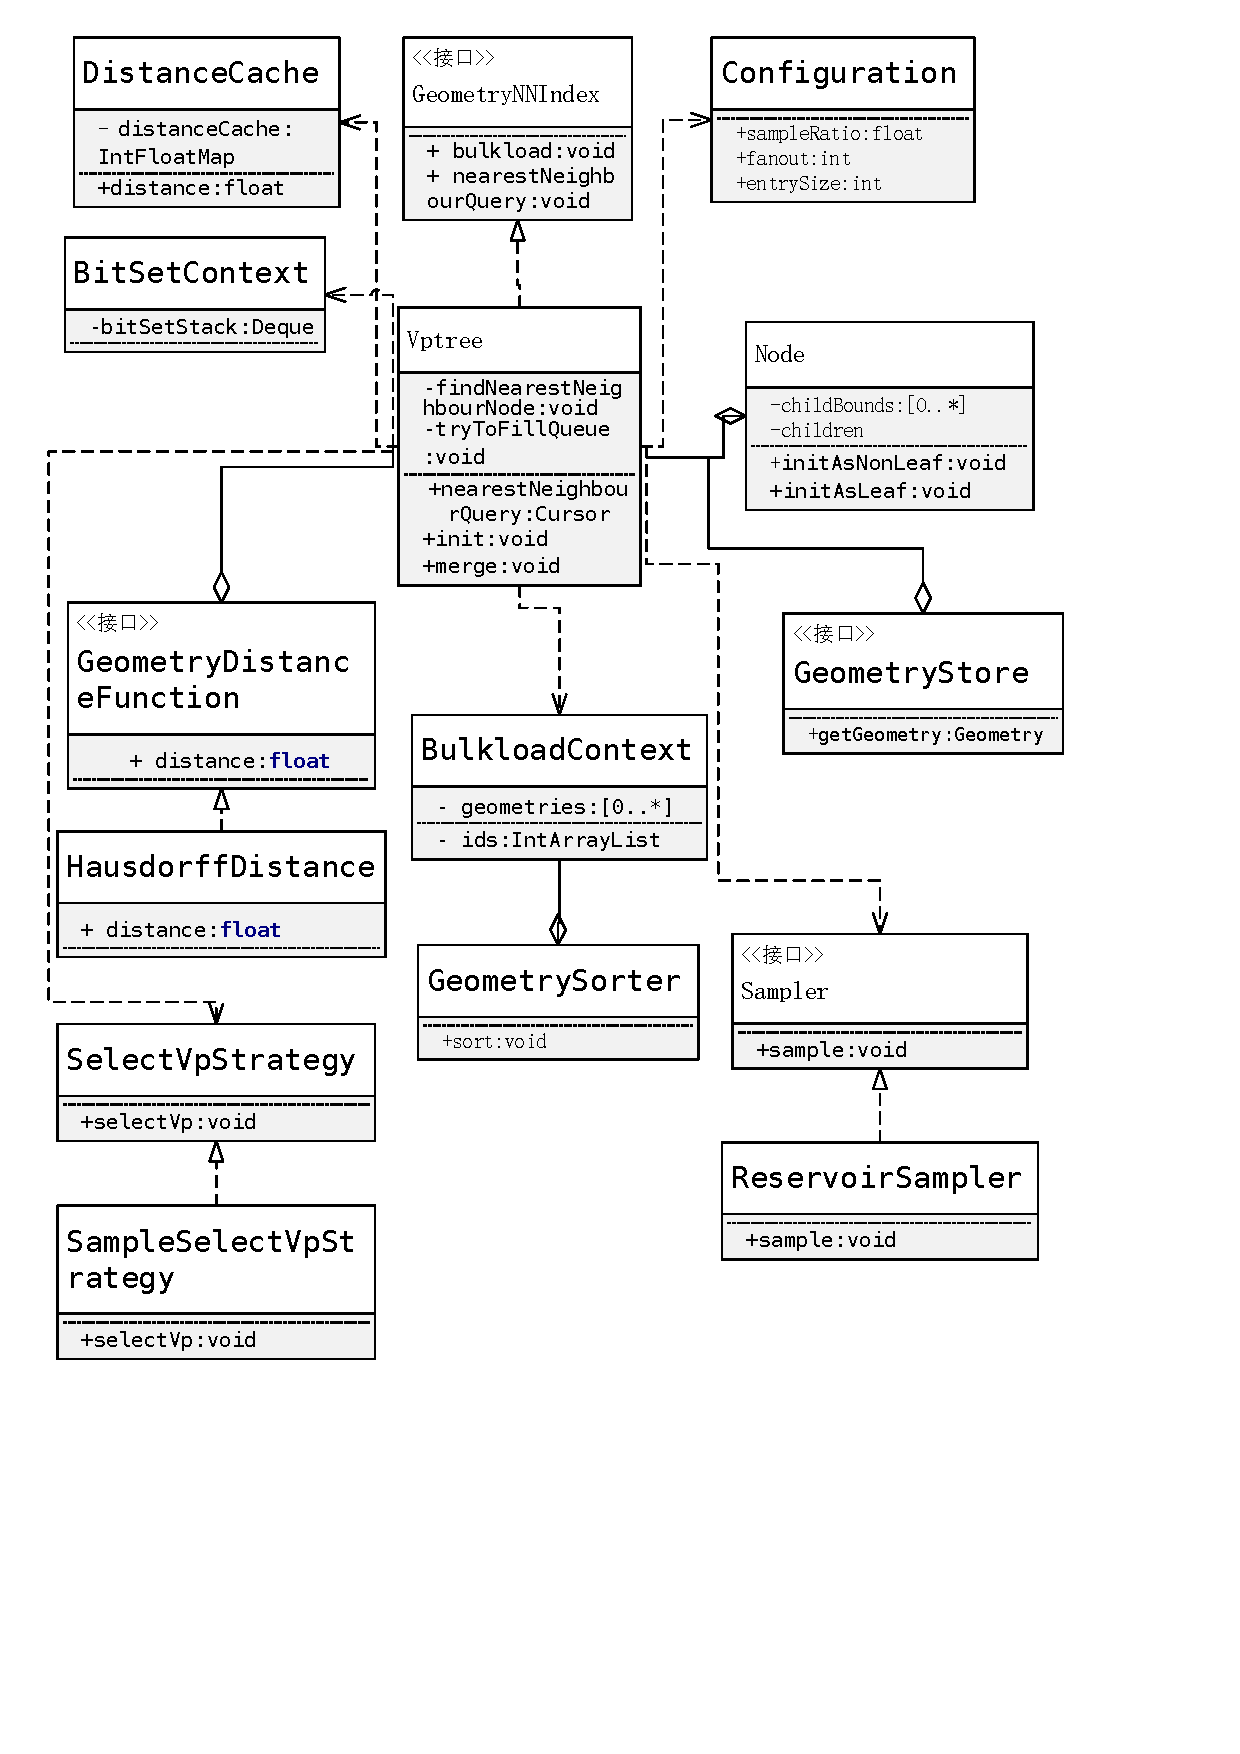
\includegraphics[width=6in]{new_FIGs/chapter4/vp-tree-general-structure.pdf}
  \caption{优先点树索引类图}\label{vp-tree-general-structure}
\end{figure}

DistanceCahce是对距离的缓存结构,以减少数据点之间距离的计算次数。它其实是一个针对特定轨迹的缓存结构,一个DistanceCache保存其他若干轨迹相对于目标轨迹的距离。所以在代码实现中,会有多个DistanceCache保存在内存里。为了避免在使用时一一遍历寻找特定轨迹的DistanceCache,本文在检索过程中保持DistanceCache 的栈与轨迹栈一一对应,从而顺序读取各个轨迹的cache,这在运行时消耗了相当数量的内存。

BitSetContext用于记录VpTree一条检索路径中各个非叶节点的分支已搜索状态,用于避免重复检索。与distanceCache一样,BitSetContext以通过顺序上的一一对应关系来维护和节点之间的对应性。而且目前BitSetContext 的实现中,依赖于外部的释放内存空间,BitSetContext本身没有设计垃圾回收机制。

Configuration类用于保存VpTree的元信息,例如扇出数,最小扇出数,取样方法,节点尺寸,采样率等。这个参数是VpTree的固有属性,在检索和插入操作中,都被使用到。

BulkLoadContext是VpTree初始建树时的输入参数,主要包括一个docIdList和一个Geometrylist,其主要功能是在初始建树的过程中提供数据.
GeomtrySorter 是一个排序工具类,用于对BulkLoadContext中的轨迹进行排序,以应对初始化建树时的多路切分,这个类是对快排的扩展实现。

GeomtryDistanceFunction是VpTree数据点间距离计算的接口,本文实现的算法HausdorffDistance采用豪斯多夫距离,但这显然不是唯一一种距离衡量方式。因此预留接口,以备扩充。

SelectVpStrategy是VpTree用于选择优先点的策略接口,本文目前只支持最大标准差的选取方法。其实,随机取优先点也是一种可选方式。Sampler是取样器的实现类,在最大标准差SampleSelectVpStrategy的实现中,使用了采用器进行采样,目前的采样器的实现只有一种ReservoirSampler。

综上所述,整个VpTree结构的设计,是充分面对扩展的。对于未来可能出现的新的距离计算函数,采样方式,节点结构,数据点形式,有良好的适应性。只是在内存使用上,存在一定的瑕疵,这在未来版本的优化中会得到解决。


\subsection{优先点树节点结构}
本文所设计实现的优先点树的结构是对最简单vp-tree结构的改良,将原生vp-tree的两路结构改为多路结构。相应地,就需要把按中值进行二分修改为以边界值进行多分,并且为了提高检索的速度,减少检索时的距离运算量,改良后的vp-tree的非叶节点不仅存储了Vantage Point ID和每棵子树的指针,还存储了每个子树的距离值的上界和下界以及最大距离值。具体结构见图~\ref{vp-tree-structure1}所示为一个4路vp-tree的内部结构示意图。
\begin{figure}[H]
  \centering
  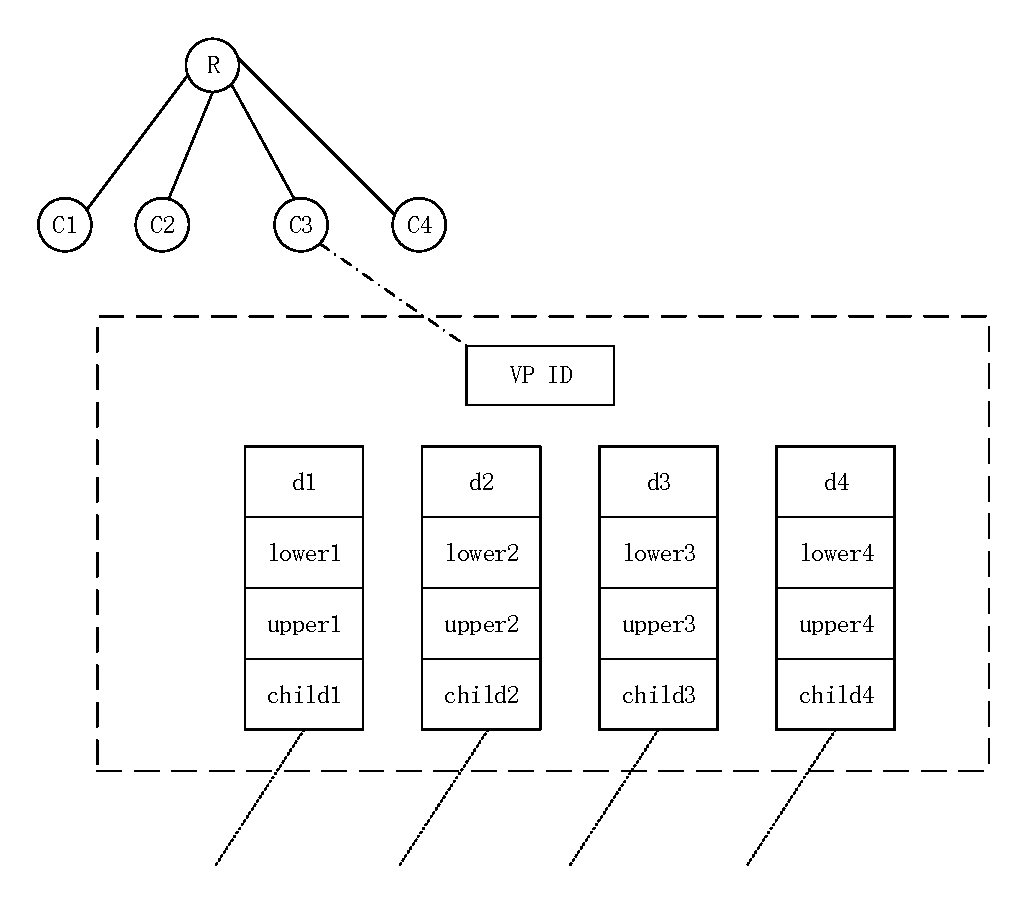
\includegraphics[width=5in,height=3in]{new_FIGs/chapter4/vp-tree-structure1.pdf}
  \caption{4路vp-tree的内部结构示意图}\label{vp-tree-structure1}
\end{figure}
\subsection{初始建树的流程}
初始建树的输入数据是一系列的docId+Geometry,初始建树的输出是一棵完整的多路vp-tree。具体流程见~\ref{create-node-flow}。\textbf{注意:本文用DP来表示Data Point,即数据点,用VP来表示Vantage Point,即被选做优先点的数据点,用Node来表示vp-tree的节点。}

如图所示初始建树实际上是一个递归的过程。但是为了避免出现内存溢出,本文选择了用循环+栈的模式。流程开始时,首先将根节点压栈,然后判断数据点的个数是不是小于叶节点的数据量标准。如果是,就意味着已经达到终止这一分支的条件,则直接初始化为叶节点,然后通过空流程返回循环判断。如果数据量仍然大于叶节点的数据量,就使用选取函数选择优先点,计算其他各个数据点到优先点的距离,再根据距离进行升序排序。\textbf{注意:由于此时有一个点被选做优先点,所以数据点总量要减一},然后判断剩余的数据量是否大于扇出数,如果数据量已经不能满足全部的扇出,那么就初始化为单个非叶节点入栈,从而进入下一次循环。如果数据量依然足够分割全部的扇出,就按照距离排序的结果进行多路切分,用新建的子节点代表新的子树,并入栈。将距离值,上下界值和子节点指针分别填入对应的数组中,再进入下一次循环。以此类推,循环往复,完成所有数据点的建树操作。

\begin{figure}[H]
  \centering
  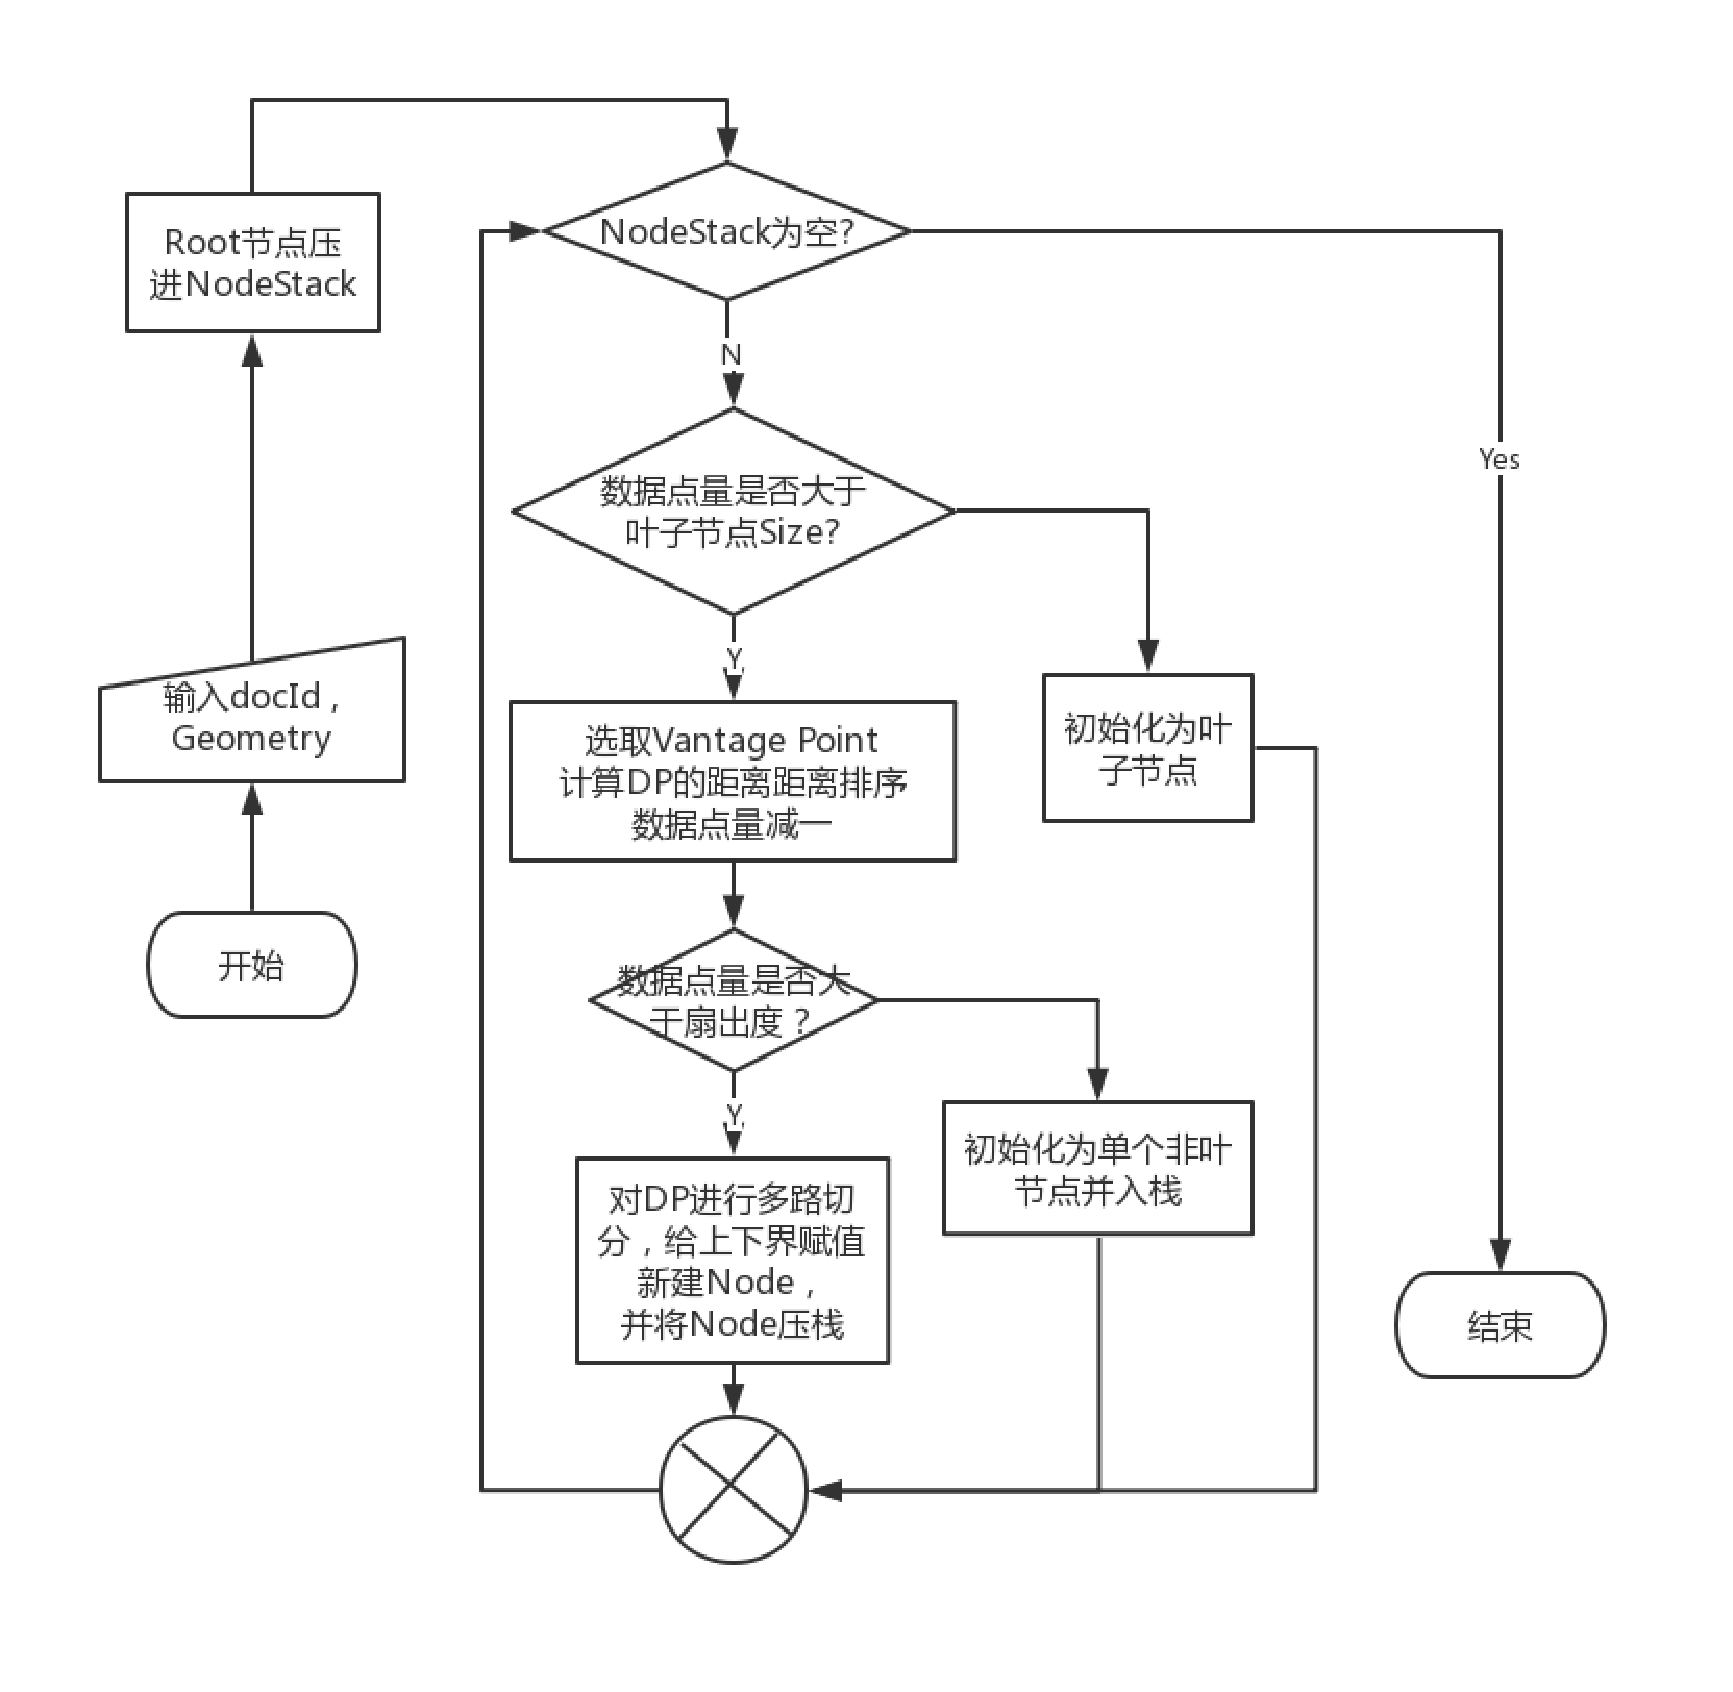
\includegraphics[width=5in,height=7.6in]{new_FIGs/chapter4/create-node-flow.pdf}
  \caption{初始建树流程图}\label{create-node-flow}
\end{figure}
\subsection{初始建树算法实现}
\textbf{注意,出于节省篇幅考虑,省略了部分简单实现}
\begin{figure}[H]
  \centering
  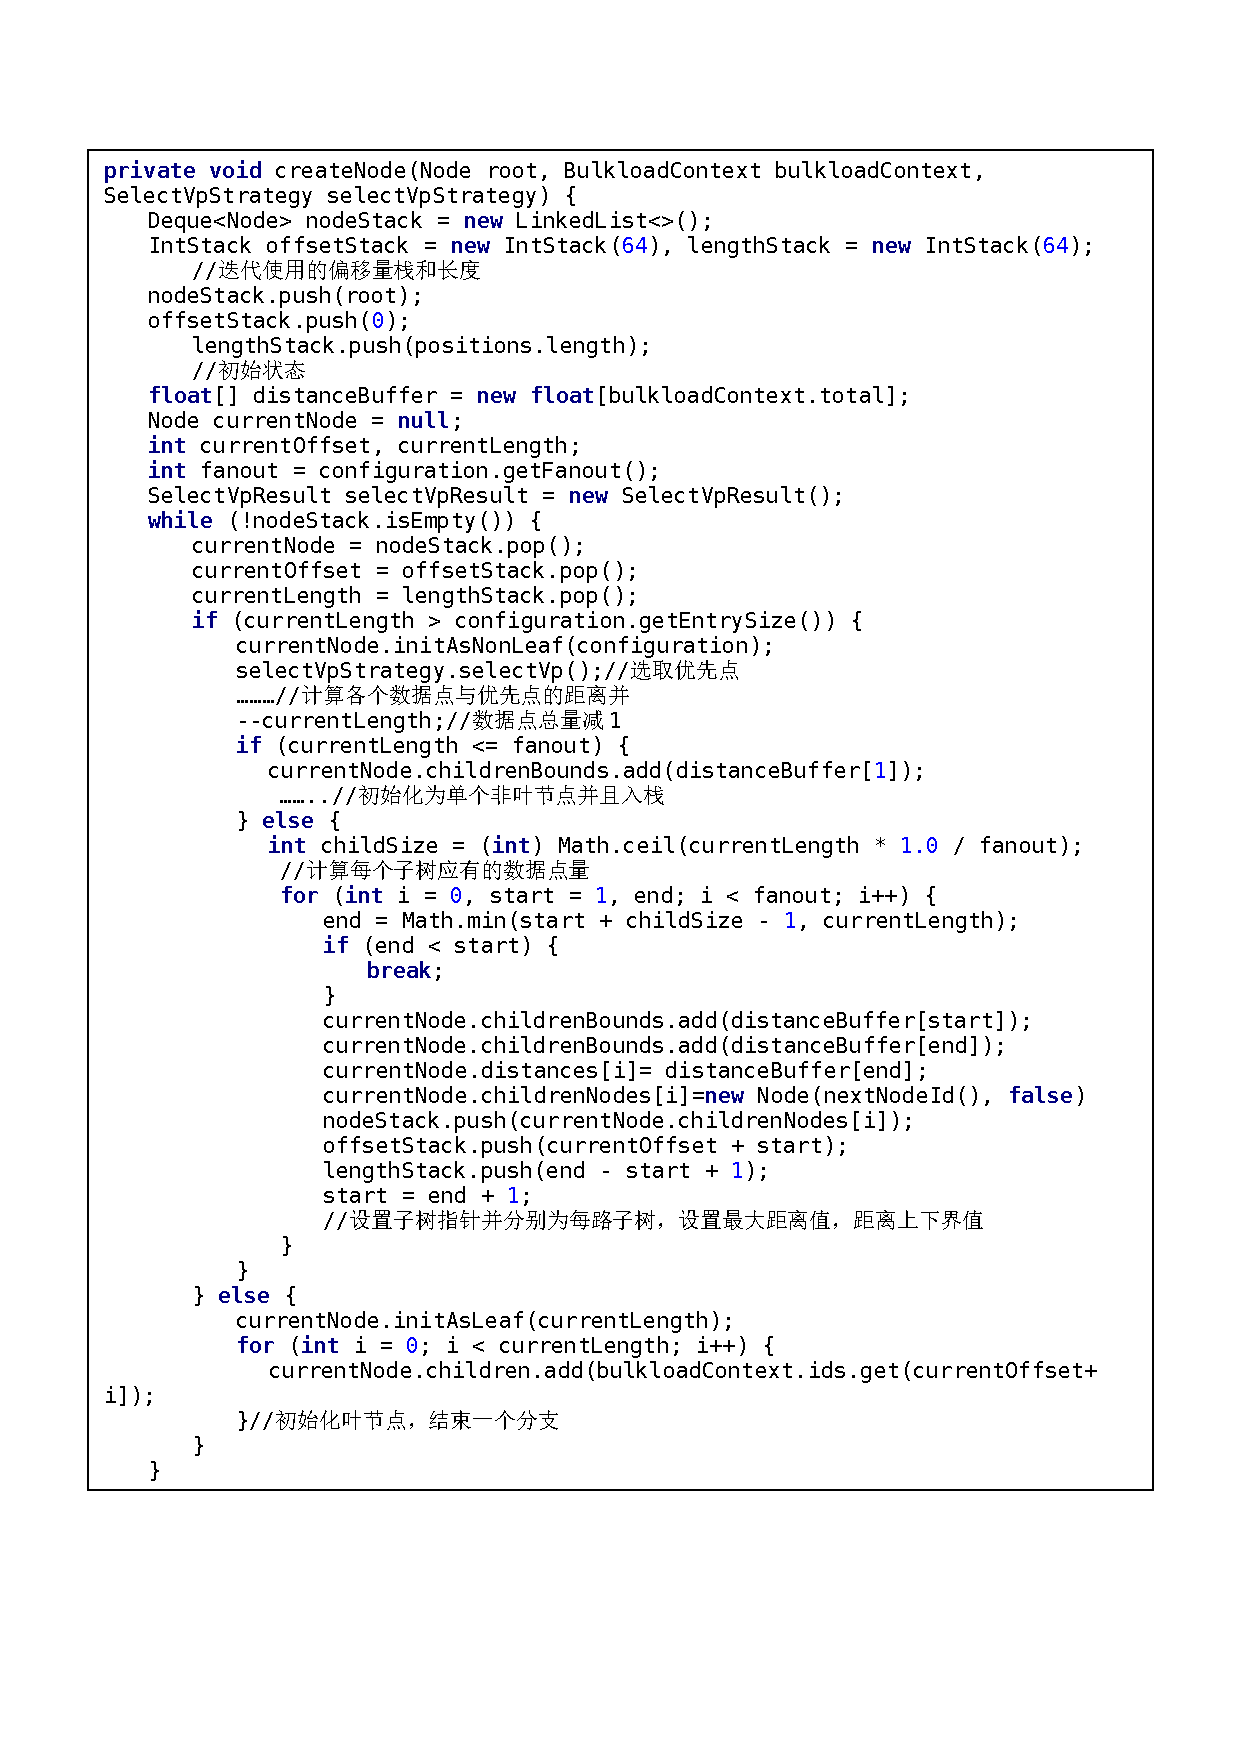
\includegraphics[width=6in,height=7.6in]{new_FIGs/chapter4/initVpTree-code.pdf}
  \caption{初始建树代码}\label{create-node-code}
\end{figure}
\subsection{设计要点}
\textbf{设计要点1:优先点的选择算法:}

在初始建树的过程中,优先点选取是非常关键的一步。选取的好坏取决于一个优先点能否让切分出来的各路子树的边界值相差足够大,因为各路子树的边界值相差越大,在检索的时候,距离值落入某一子树的边界内的可能性越大,剪枝成功的可能性越高,性能就越好。反之,如果优先点选择很差,导致多个子树的上下界非常接近,就很容易出现一个距离值可能在多个子树中搜索的情况,造成性能下降。因此,如何选择尽可能优的优先点,是算法实现的重点。
\begin{figure}[H]
  \centering
  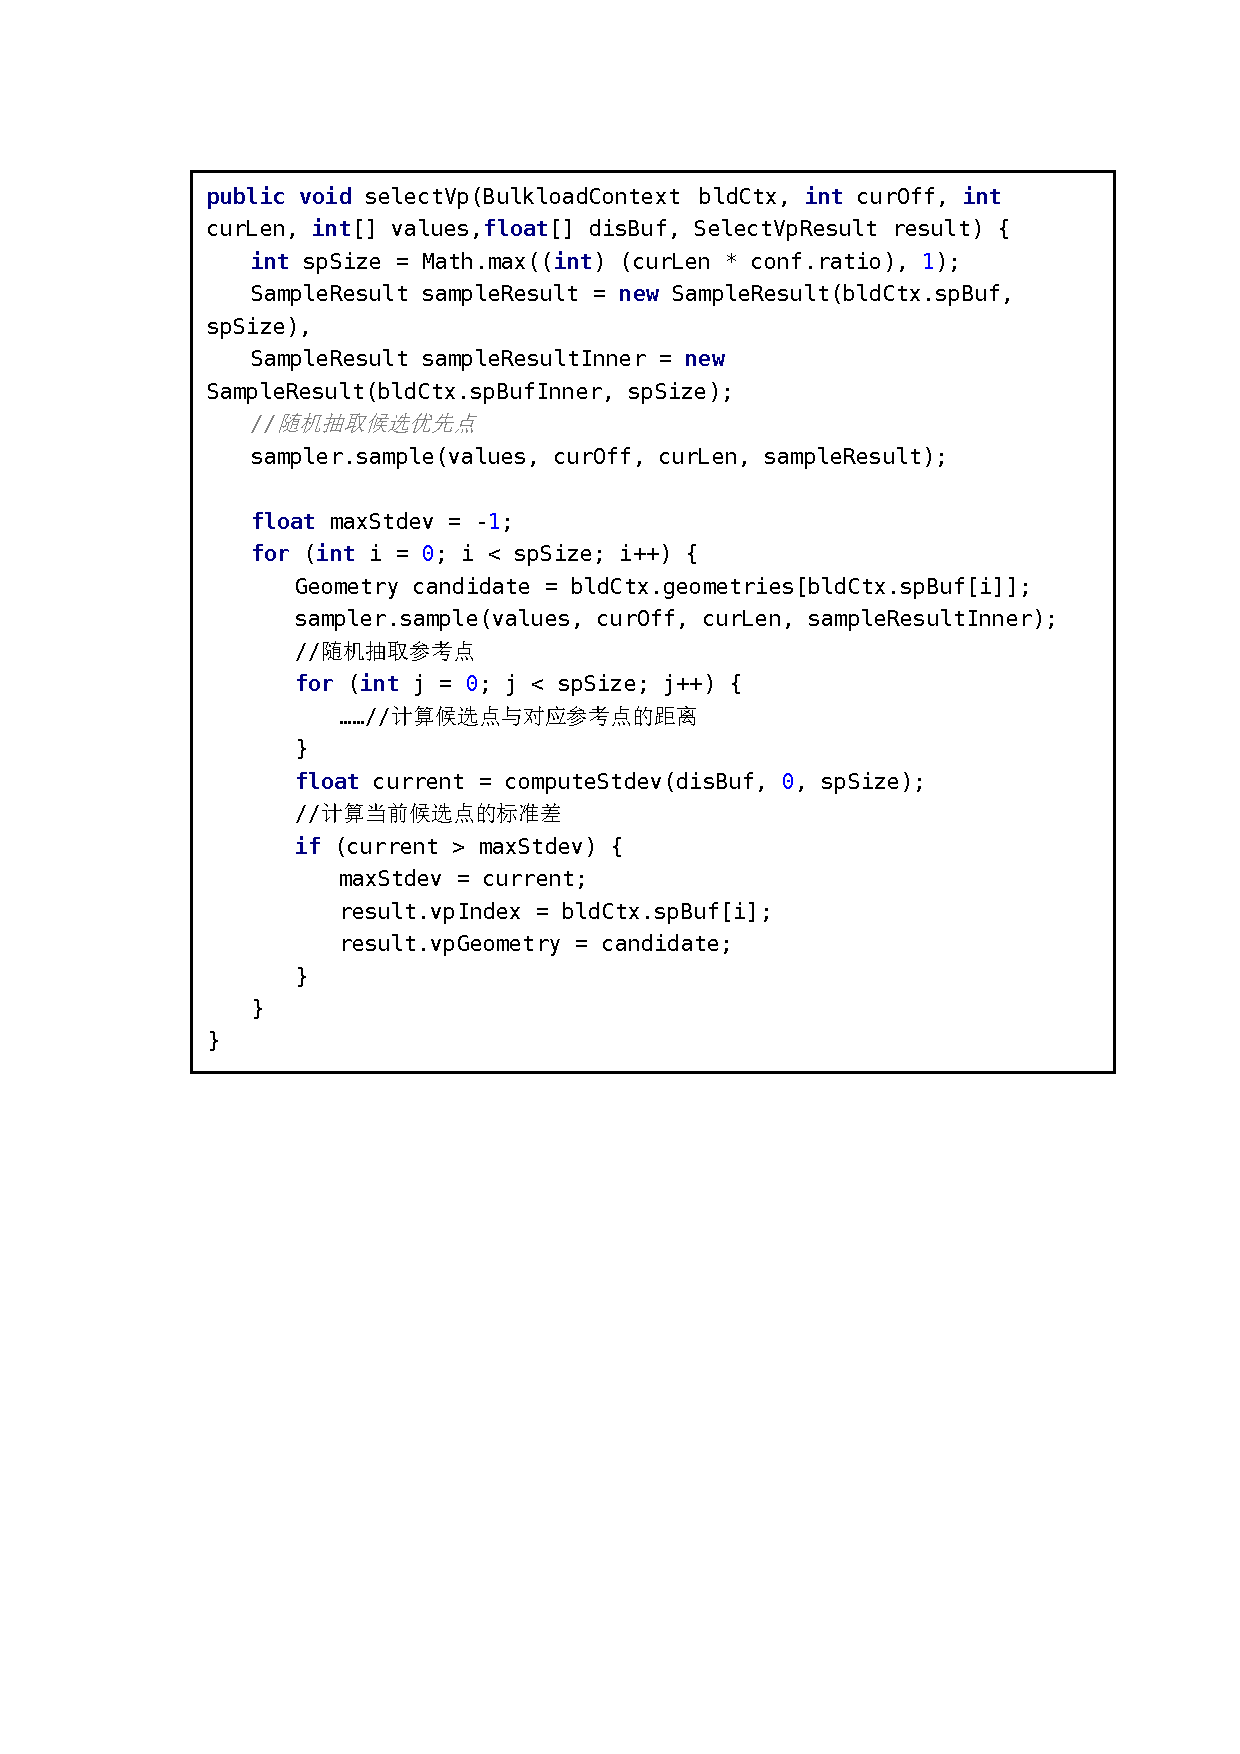
\includegraphics[width=6in,height=5.5in]{new_FIGs/chapter4/select-vp-code.pdf}
  \caption{优先点选取代码}\label{select-vp-code}
\end{figure}
本文针对优先点选择的实现是基于随记取样和标准差结果的。本文认为,一个点与其他点距离的标准差越大,作为优先点的性能越好。而由于数据全量很大,不可能都计算,就采用随机抽样的方式进行。其设计思路是,在数据点全集中随机取样K 个点,作为候选的优先点。针对这K 个候选的优先点进行循环遍历,每个候选优先点再随机取K 个点作为参照点,然后计算每个候选优先点和参考点之间距离的标准差,最后取标准差最大的那个候选点作为真正的优先点。这样的选举过程涉及到取样,距离和标准差的计算,相当于用一部分初始建树性能的降低来换取了检索性能的提高。具体实现如图~\ref{select-vp-code}所示。

\textbf{设计要点2:使用长度栈和偏移量栈记录内存状态,避免冗余内存:}
初始建树的输入数据是两端段很长的数组,分别保存了docID和对应的Geometry。为了减少内存使用,本文采用偏移量+长度这样的组合量来记录每个节点所涉及的数据状态,从而避免了输入数据的内存复制。另外,由于使用了栈实现,在多路划分的过程中,优先级是从右向左,而且是深度优先的。也就是说优先点树的最右边一个分支会最早完成创建。\textbf{由于vp-tree的多路切分是均衡的,所以vp-tree自然是一个平衡树,分支初始化的顺序与最终结果没有关系}。

\section{相似轨迹检索功能模块详细设计}

\subsection{KNN问题的定义和解决思路}
在我们的轨迹数据服务的作用域内,KNN问题,即K Nearest Neighbour的含义是,找到与目标Geometry距离最近的K个Geometry。

原生vp-tree的搜索算法是面对NN问题,也就是nearest Neighbour问题,只找一个距离最近的点。那么面对KNN问题,显然不能通过简单地运用K次原生搜索算法来解决,那样会导致接近三次方级别的消耗,这是用户绝不会接受的。

比较直观的想法是,使用一个大小为K的最小堆,在搜索过程中实时更新这个最小堆的状态,那么在搜索算法走完的时候,这个最小堆中的结果就是K个距离最近的Geomtry。这是\cite{DBLP:journals/vldb/FuCCM00}中所阐述的思路。本文实现的算法的借鉴了这一思路,同样是用堆来动态维护状态,但采取了一些措施应对这一思路的明显短板以获取更好的检索性能。详见下节。

\subsection{设计焦点与思路概述}
在KNN问题的搜索过程中,对于每一个多路节点,除了考虑与优先点的距离之外,还要考虑一个容忍距离T,也就是超出这个容忍距离T的数据点不再予以考虑。
\cite{DBLP:journals/classification/ProencaN17}
\begin{figure}[H]
  \centering
  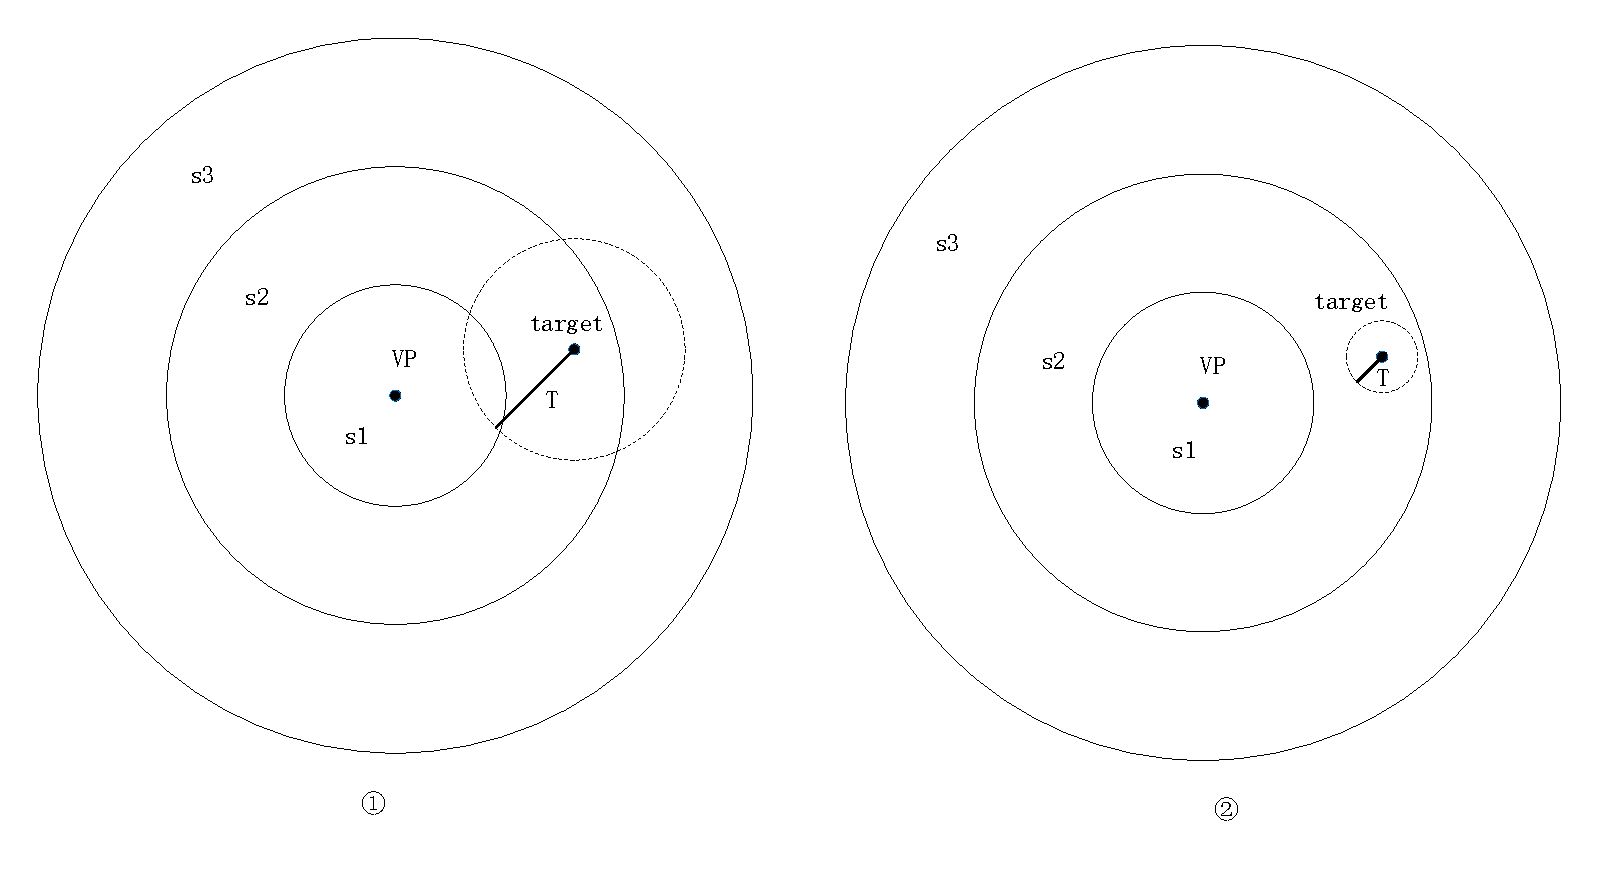
\includegraphics[width=6in]{new_FIGs/chapter4/thredhold.pdf}
  \caption{容忍距离对剪枝的作用示意图}\label{thredhold}
\end{figure}
这是距离范围剪枝的基本依据。如图\ref{thredhold}所示,某一数据空间基于优先点VP被分为S1,S2,S3三个子空间,目标轨迹target落在子空间s2中,T为容忍距离。在①情况下,容忍距离T的半径范围覆盖了S1,S2,S3,使得检索必须遍历全部三个分支。而对于②而言,T半径仅仅只在S2子空间内,所以可以认定,S1和S3中不可能包括与target距离小于T的点,从而排除S1,S3,实现剪枝。显而易见的是,容忍距离越小,成功剪枝的概率越高,检索性能越好。但是如果容忍距离太小,又可能过度剪枝造成检索不到结果。所以容忍距离的初始值和收敛速度是直接影响检索性能的关键。\cite{DBLP:conf/hucc/ZengLJLCM14}

在上文所述的单纯用最小堆动态更新检索结果的算法中,其最大问题在于,容忍距离是从正无穷开始更新的。这使得检索从一开始完全不可能做到剪枝,大量的分支都被搜索了。容忍距离的收敛速度会非常慢,导致剪枝的效率很低,性能也比较差。

基于上面所提到的容忍距离收敛较慢问题,本文采用了结果堆预填+回溯的方式进行优化处理。即通过原生vp-tree搜索算法,先找到single nearest neighbour,在这个过程中预填结果堆,并保存从root到single nearest neighbour的整条路径的所有节点。以结果堆中最大距离作为容忍距离的收敛起点,再回溯整条路径中的节点,完成检索。这样通过预先填结果堆,使得容忍距离以更低的起点收敛,使得很多分支在检索开始阶段就被剪掉,容忍距离收敛的速度更快,性能更好。
\subsection{检索算法流程图}
如图\ref{search-flow}所示为检索算法的运行流程图。
\begin{figure}[H]
  \centering
  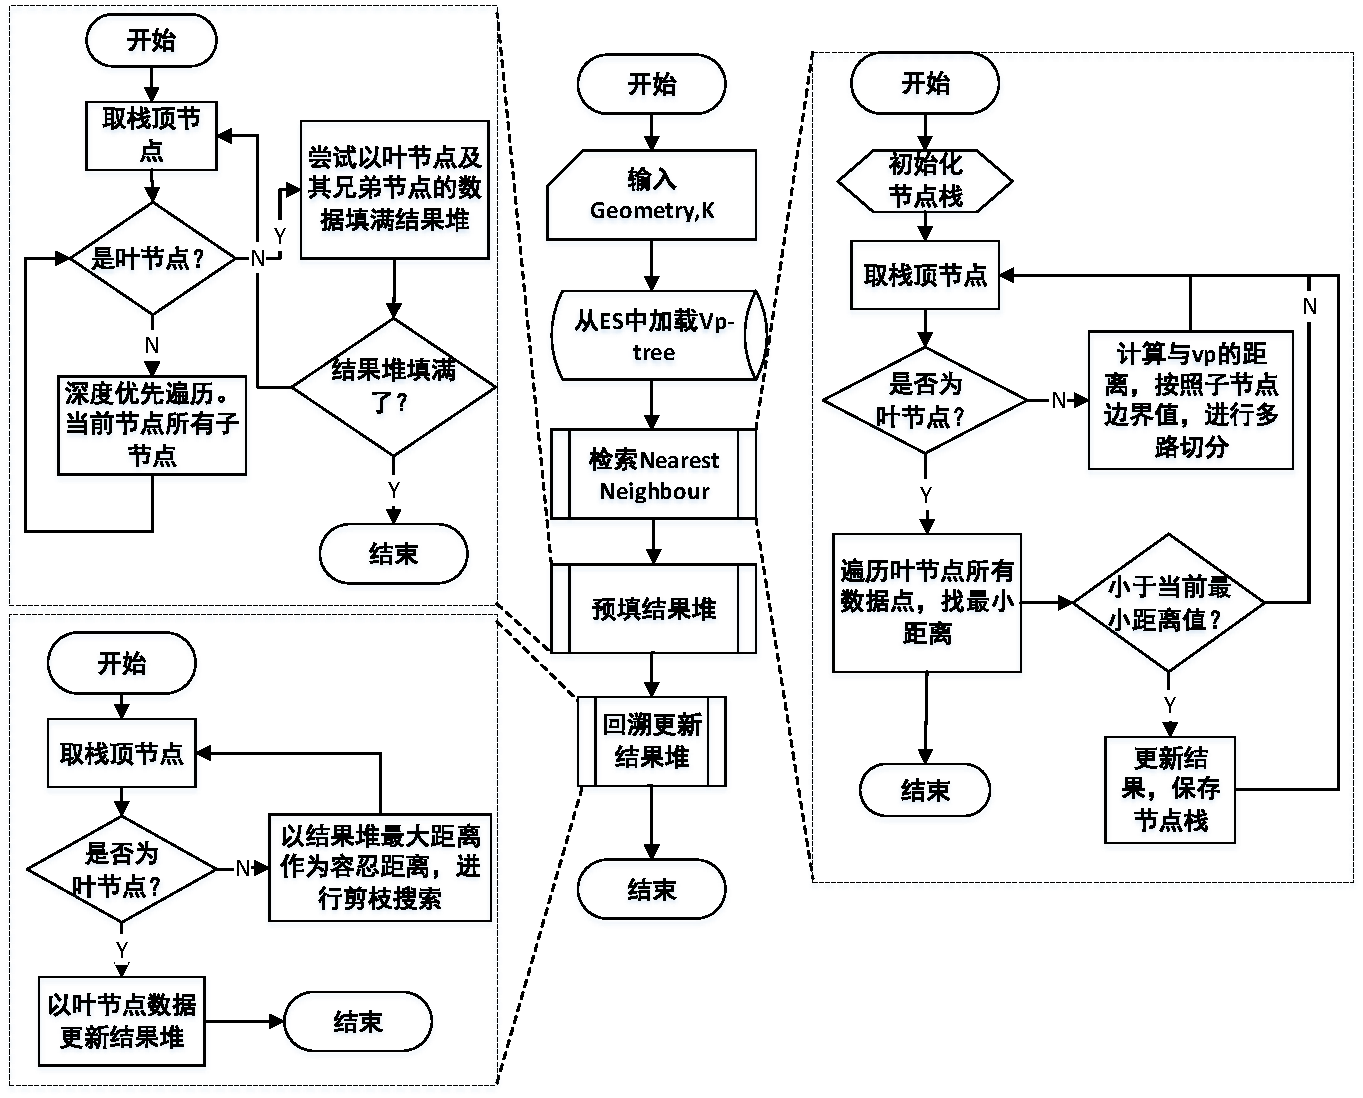
\includegraphics[width=6in,height=5.2in]{new_FIGs/chapter4/search-flow.pdf}
  \caption{检索算法流程图}\label{search-flow}
\end{figure}

\subsection{相似检索功能各子流程代码实现}
本节将会依次展示\ref{search-flow}中所示的各个子流程的代码实现。

\textbf{检索最近邻居代码实现:}
\begin{figure}[H]
  \centering
  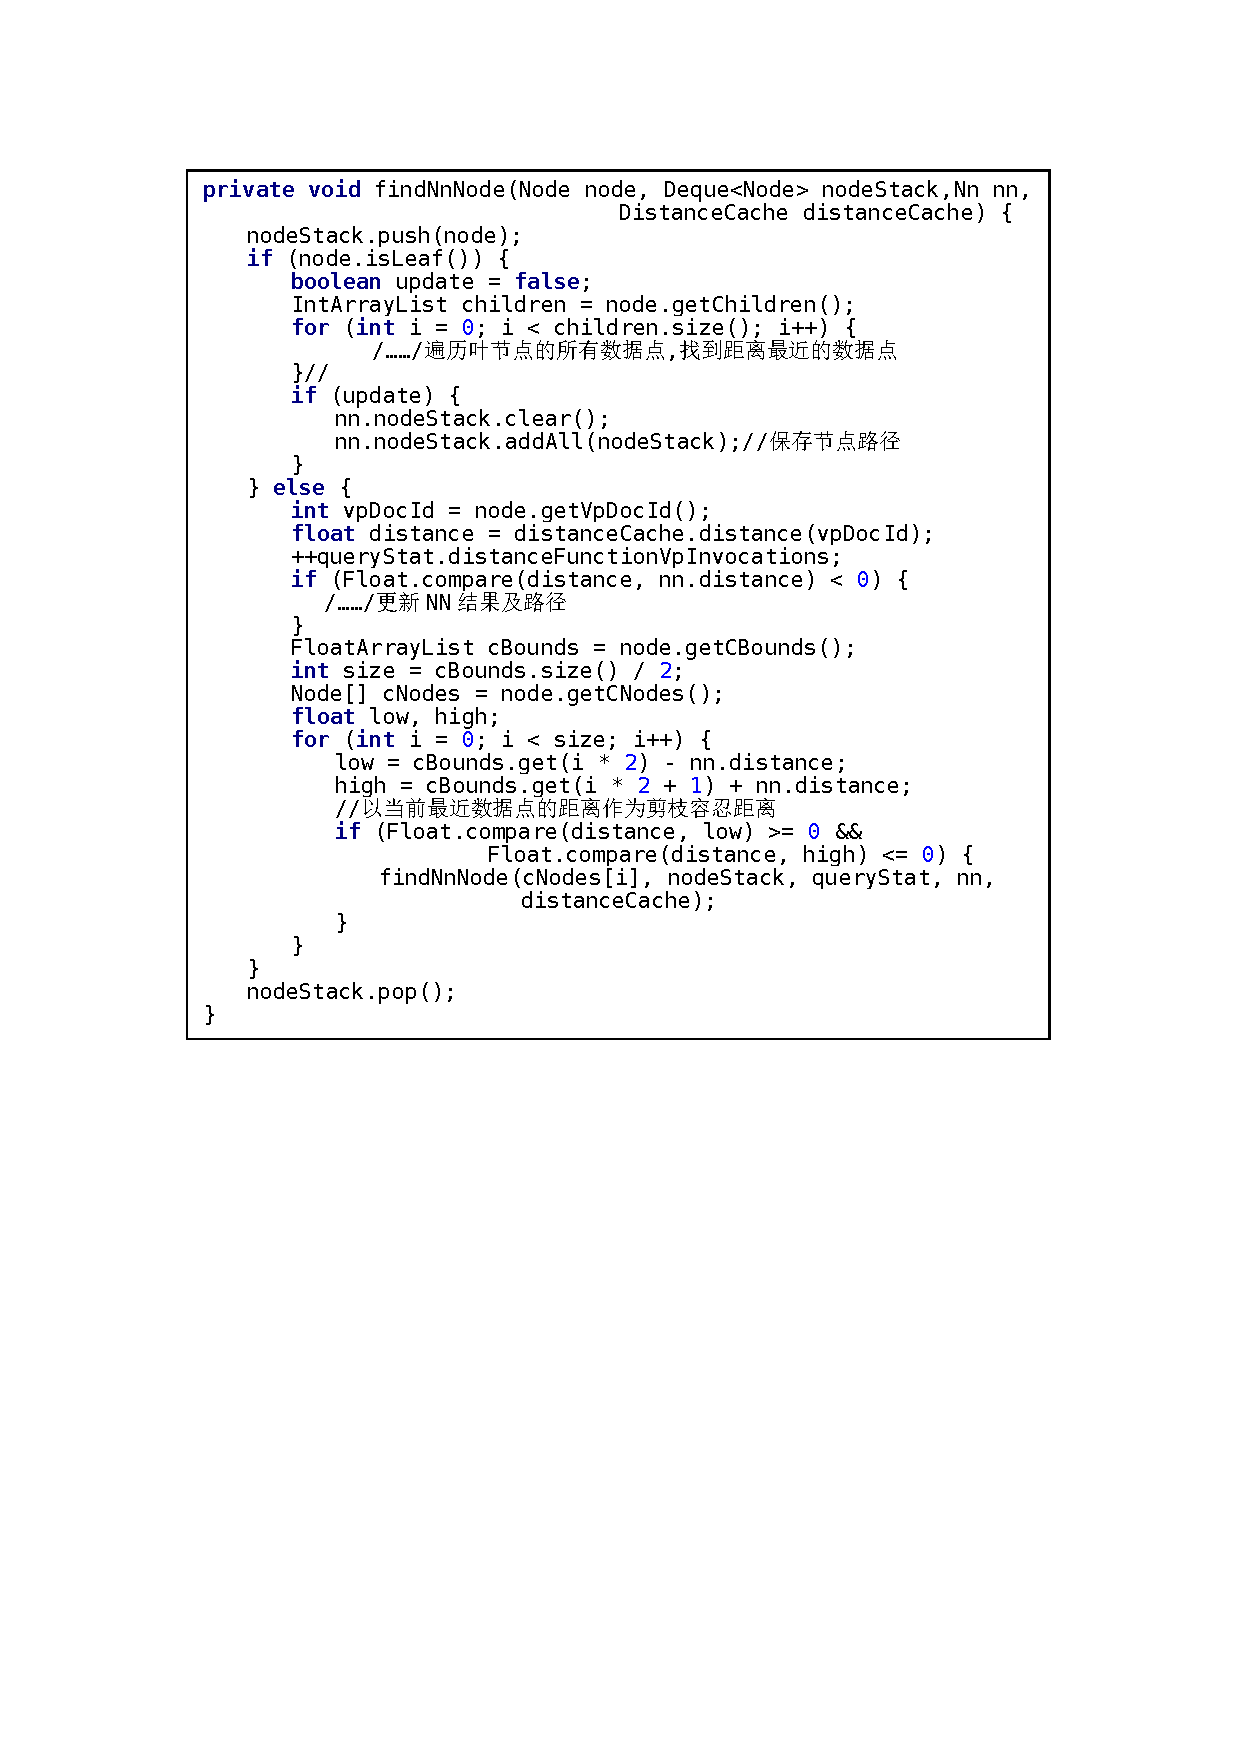
\includegraphics[width=5.8in,height=5.5in]{new_FIGs/chapter4/findnn-code.pdf}
  \caption{检索最近邻居代码实现}\label{findnn-code}
\end{figure}

\textbf{预填结果集代码实现:}
\begin{figure}[H]
  \centering
  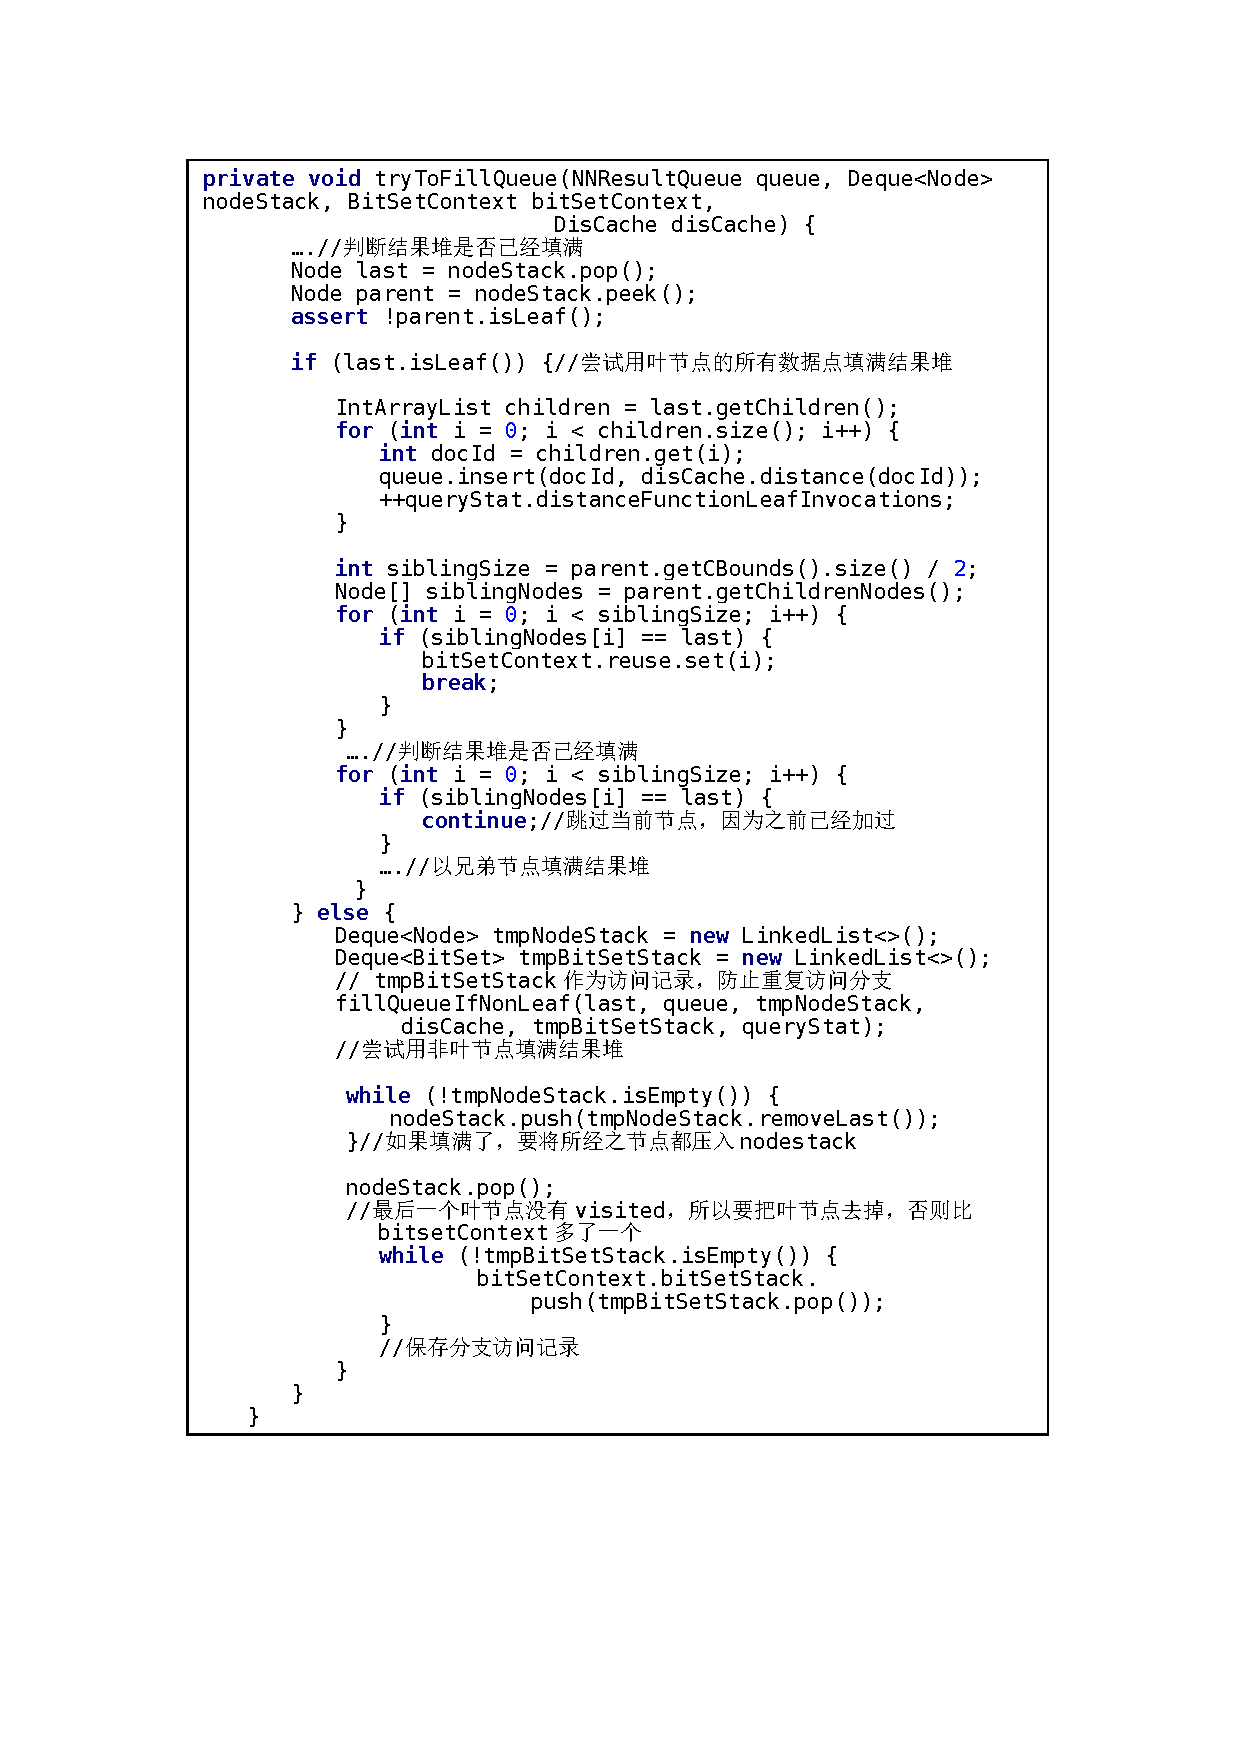
\includegraphics[width=5.8in,height=7.8in]{new_FIGs/chapter4/trytoFillQueue-code.pdf}
  \caption{预填结果集代码}\label{trytoFillQueue-code}
\end{figure}
\subsection{相似检索功能实现要点:避免重复访问}
在当前的索引实现中,由于经历了预填结果集的操作,某些节点的一部分分支在预填过程中就已经被搜索过了。因此,在回溯过程中,如果不加甄别,可能会重复遍历相同的分支,导致性能损失。关于这一点,本文使用了BitSet 栈的方式来实现,在预填结果集的过程中,与节点栈同步保存一个Bitset栈,两者的顺序一致。每个bitset与vp-tree 的扇出数一致,用于保存若干分支中,哪些已经被访问过了。这样,在回溯发生的时候,首先检查对应的bitset,对于那些已经被置位的分支直接跳过,只访问尚未遍历过的分支,避免重复的检索和距离计算。

\section{插入新轨迹功能模块详细设计}
\subsection{Insert操作算法概述}
在系统运行过程中,经常出现新的轨迹数据被插入已有索引的情况。这种情况下,如果每次都是将整个数据点集合重新进行初始建树,消耗会非常大。因此,有必要实现优先点树插入节点的相关算法。

对于新数据点插入操作,首先要进行深度搜素,找到正确的叶节点,然后对应以下几种情况分别采取不同措施。

第一,新插入的数据点所匹配的叶节点未满,则直接插入到正确的叶节点的空槽位中。如图\ref{insert-show0}所示,新数据点e被插入叶节点L的空槽位中。这种情况下,只有数据赋值操作,没有距离计算,性能最好,之后几种情况的处理原则都是使后续插入尽可能满足第一种情况。注意,必须保证叶节点中数据点的顺序性,所有相关元信息的对应位置都要向后移动。

\begin{figure}[H]
  \centering
  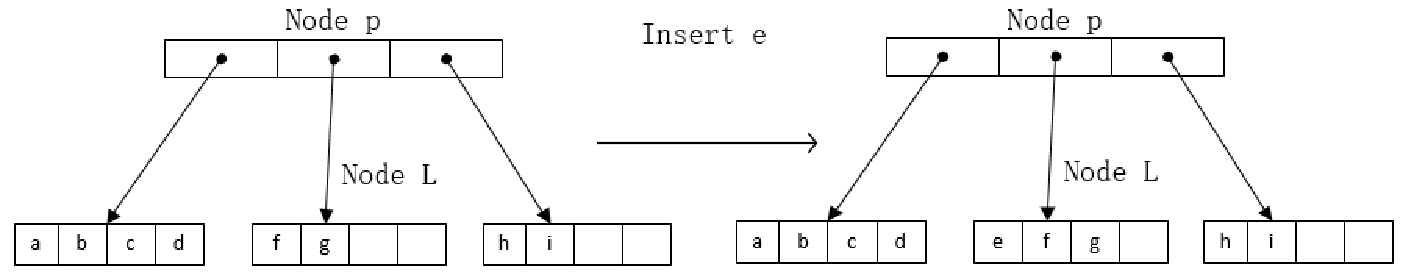
\includegraphics[width=6in]{new_FIGs/chapter4/insert-show0.pdf}
  \caption{直接插入对应叶节点算法示意图}\label{insert-show0}

\end{figure}
第二,新插入的数据点所匹配的叶节点已满,但是其父节点分支数未满。则分裂匹配的叶节点,为父节点新增子叶节点,并且进行数据移动。注意,分裂之后的数据重分布应该秉持均分的原则,让空槽位尽可能均匀地分配在两个叶节点中,从而使得后续的插入操作尽可能多地符合叶节点不满的情况,避免发生连续多次分裂的情况。如图\ref{insert-show1} 所示,数据点e本应插入在节点L的f之前,但是因为节点L已经满了,而节点P的分支数未满,此时将节点L分裂成两个新节点L2 和L3,将节点L中原本相距节点P的优先点距离最远的数据点h,i分配给L3。以此实现了数据点e的插入。同时保证L2,L3两个叶节点都有空槽位,以备后面的插入操作。

\begin{figure}[H]
  \centering
  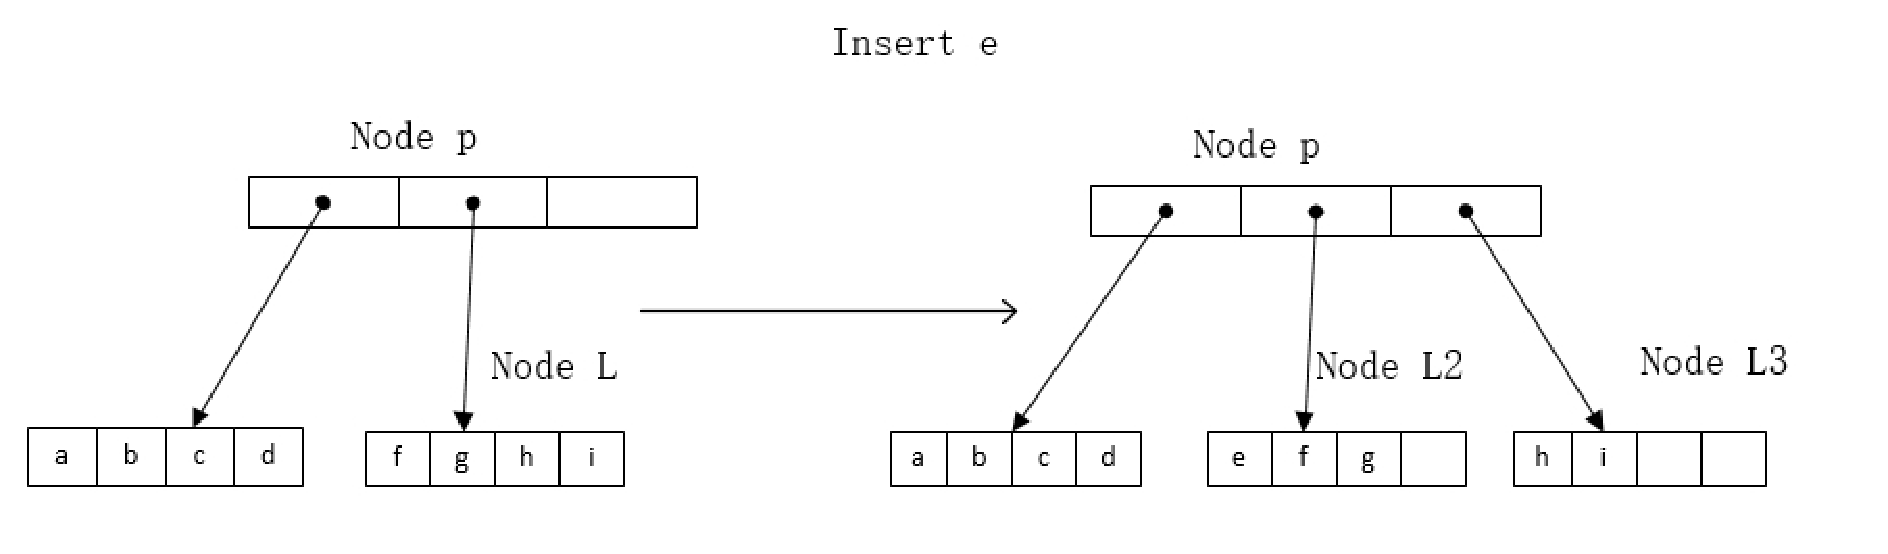
\includegraphics[width=6in]{new_FIGs/chapter4/insert-show1.pdf}
  \caption{叶节点分裂算法示意图}\label{insert-show1}
\end{figure}

第三,新插入的数据点所匹配的叶节点已经满了,而且父节点的分支数也已经满了,不能再分裂出新的叶节点。这种情况下,采用\textbf{中心扩散}的方式寻找最临近未满的兄弟节点,进行数据重分布。注意,这里要考虑距离和空槽位数量两种因素。空槽位数量越多的叶节点,重分布之后空槽位分布越均匀,越适合进行数据重分布。但是重分布不只是涉及目标叶节点和兄弟叶节点,而是涉及到两者之间的所有叶节点。两者之间的距离越远,需要重新分布的节点数就越多,消耗越大,反之,消耗越小。所以此处应该以距离最近为优先,以最小化指针移动和元数据更新的消耗。在距离相同的情况下,根据叶节点空槽位的数量决定,空槽位越多的兄弟节点,越优先。如图\ref{insert-show2}所示数据点以本应插入到节点L2 中,L2已满,则以中心扩散的方式,同时发现了两侧距离相同的未满节点L1和L3,此时发现L3中的空位比L1中多,因此选择L3进行数据重分布,完成e的插入。

\begin{figure}[H]
  \centering
  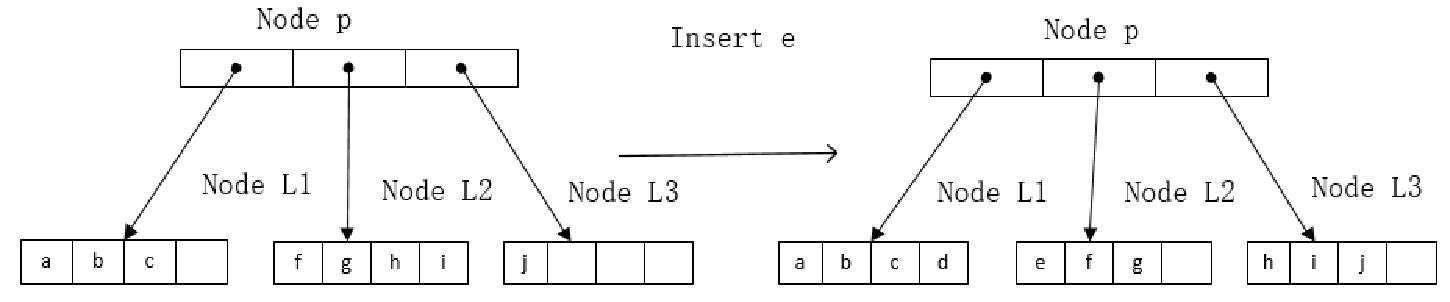
\includegraphics[width=6in,height=1in]{new_FIGs/chapter4/insert-show2.pdf}
  \caption{叶节点数据重分布算法示意图}\label{insert-show2}
\end{figure}

第四,新插入的数据点所匹配的叶节点,父节点以及所有的兄弟节点都已经满了,则向上回溯,找到第一个未满的祖先节点,如祖先节点的分支数未满,则优先进行目标分支的分裂,形成新的分支。
\begin{figure}[H]
  \centering
  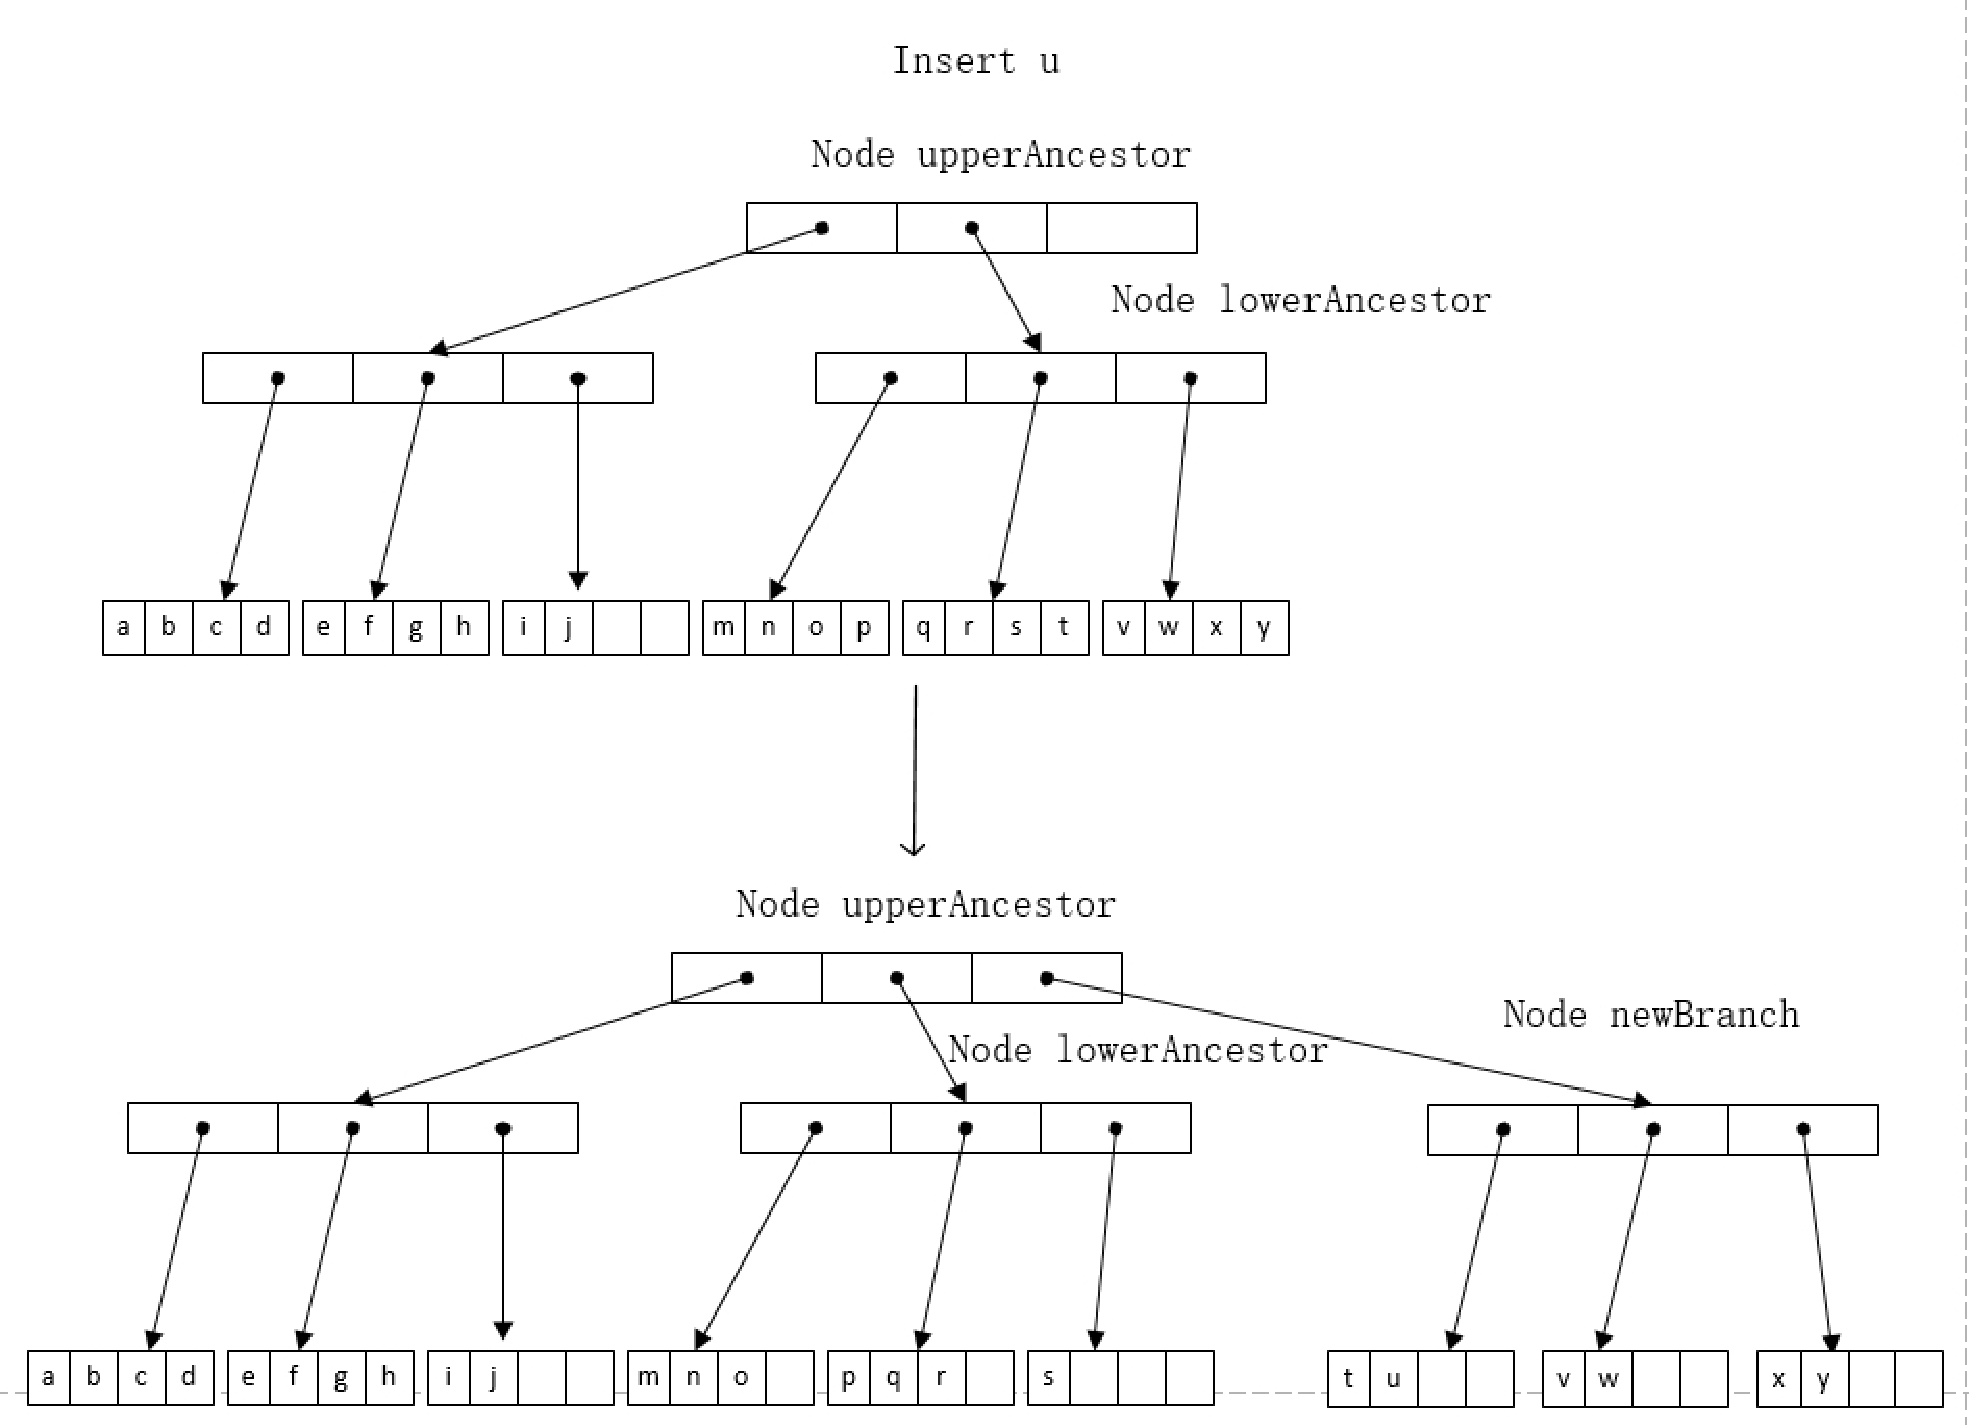
\includegraphics[width=6in,height=4in]{new_FIGs/chapter4/insert-show3.pdf}
  \caption{分支分裂算法示意图}\label{insert-show3}
\end{figure}
\textbf{注意,在这种情况下,不能像叶节点数据进行简单的移动就解决问题,由于产生新分支意味着必须重新建立子树,才能将原分支的数据点和新数据均匀分开,以降低接下来插入操作的负载。}如图\ref{insert-show3}所示,当插入数据点u的时候,分裂节点lowerAncestor,产生节点newBranch,并将均分的数据集合分别建立新的叶节点。

\begin{figure}[H]
  \centering
  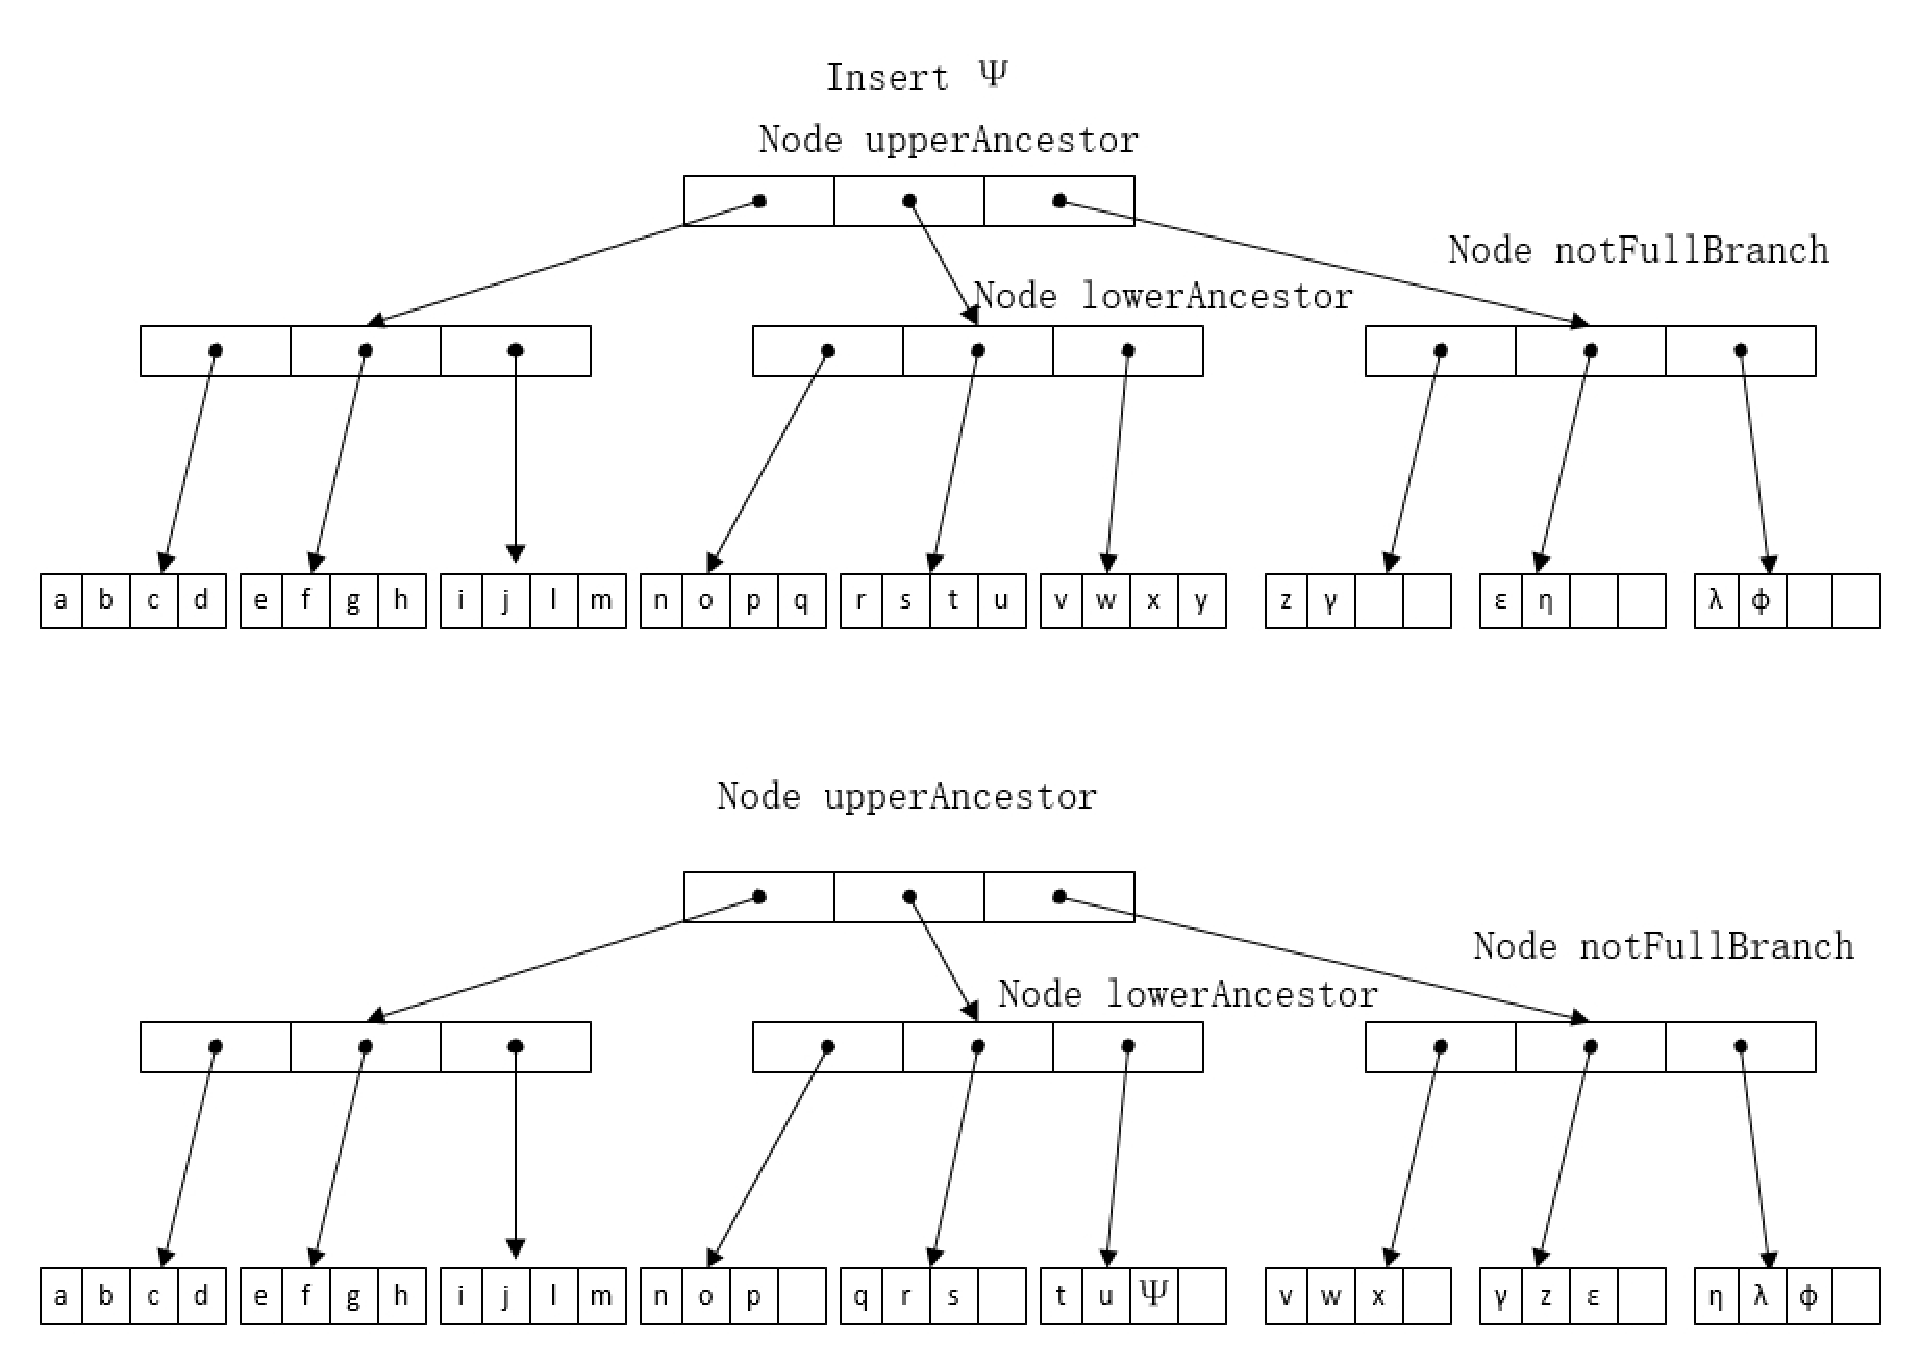
\includegraphics[width=6in,height=5in]{new_FIGs/chapter4/insert-show4.pdf}
  \caption{分支重分布算法示意图}\label{insert-show4}
\end{figure}
第五,如果祖先分支数已经满了,则寻找分支数据未满的子树的祖先进行数据重新分布。与分支分裂不同的是,分支之间的数据重分布并不涉及新的数结构的生成。与叶节点的数据重分布类似,只是数据节点的移动,只是多了一个深度搜索匹配叶节点的过程。如图\ref{insert-show4}所示,当要插入节点Ψ时,发现upperAncesor的分支notFullBranch的数据点数量不满,也就是说notFullBranch的叶节点有空槽位。此时将lowerAncestor和notFullBranch进行数据重分布,以
相对于UpperAncestor的优先点的距离作为挪动数据点的依据,将那些lowerAncestor中距离较大的k项移动到notFullBranch中,这里的k是两个分支节点总数的一半与lowerAncestor现有数据点量的差值。通过将k个数据点移动到lowerAncestor,完成insert的同时,也尽可能地均匀分布了数据,为后续的insert留出空位,以尽可能地减少成本较高的数据重分布操作。


第六,如果所有的位置都已经满了,则此时优先点树已经是一棵完全二叉树。此时,进行重新建树。这种情况下,确实可以类似于情况3那样,添加一个新的根节点,然后将旧根节点作为新根节点的一个分支,再以情况三的做法进行分支分裂。但这种情况下,分支分裂的消耗等同于重新建树。

\subsection{Insert操作算法设计细节}
\textbf{Insert操作算法细节1:根节点不分裂,树的高度不变}

优先点树的插入操作,类似于B树,但是比B树的插入消耗要大很多。因为B树的值通常都是相对于一个数据原点的可排序值,而优先点树的值则是相对于不同优先点的距离。如果要进行根节点分裂,则必须要重新对所有节点的数据进行重新划分,这样的消耗与重新建树没有区别。而初始建树的过程中以最小扇出度作为终止分裂的条件,则可以留出更多空位,为下一步的插入节约计算。

\textbf{Insert操作算法细节2:以最小扇出度作为初始建树的终止条件}

这样做的目的在于推迟节点分裂的结束,使得更多的分支数目被创建出来。那么在初始建树之后,就会预留出较多的叶节点空位。当进行插入新数据点时,叶节点的空位置将会显著减少数据重新分布和节点分裂的次数,提高性能。\textbf{但是也要注意的是,最小扇出度不能设的太小,因为节点元数据的存储都是以数组方式的线性存储,如果预留过多的空位,将会导致内存消耗大大增加。所以最小扇出度的设置要衡量插入操作与内存容量而定。}

\textbf{Insert操作算法细节3:分裂与数据重分布的优先级问题}

节点分裂能够更好地创造更多的叶节点空槽位,对于连续的插入操作非常友好。而且对于分支数较多的VpTree,节点分裂将对节点元数据的更改降到2 个分支以内,实际上可以做到以少量的距离计算代替大量的内存移动和比较操作。

而数据重分布的好处在于,能够通过在节点元数据保存数据点集合的信息来实现简单的移动就能完成数据点重新平衡的效果,从而减少了新的距离计算的消耗。这在分支数少的VpTree 中性能良好。但是对于那些分支数多,跨分支范围很大的VpTree,则可能造成巨量的比较和移动操作。比如一个10路的VpTree 的,重分布的区间是从第二个分支到第八个分支,那就意味着这七个分支之间要进行数据移动。大量的比较和移动操作带来的消耗,同样可能带来性能灾难。而且如果分支的层级较高,重分布本身的距离计算也不会太少。

综上所述,节点分裂与重分布的性能消耗,与VpTree的分支数,分支距离,分支所在的层数都有关系,应该是一个动态计算的衡量结果。采用静态设置的方式,很有可能造成优先级上的偏颇,但本文出于实现的简单,静态地采用了优先分裂的原则,这显然不是性能最佳的实现。

\textbf{Insert操作算法细节4:存储数据点距离顺序}

在初始建树的同时,在节点中顺序保存当前节点数据点集合相对于上一级优先点的距离排序。这样做是为了在数据重分布的时候,避免重新的距离计算和排序,可以通过简单的数组元素移动和界标更新来完成,从而明显减少计算量,提升性能。但是这样做的代价是,重复保存了大量的id列表,消耗了额外的内存,而且在重分布的过程中,必须将顺序集合的内容进行同步更改,也带来时间消耗。而在数据点较少,距离计算量少的情况下,数据点顺序列表的存储消耗和维护成本,可能比直接进行距离计算还要严重。这其实也是一个动态衡量的策略,出于设计简单,本文对所有节点都默认采用了这种方式。

\textbf{Insert操作算法细节5:分支节点数据未满的判断}

与分支数相比,一个非叶节点所能包含的最大数据点的量与节点在整个优先点树中位置有关。位置越高,子树层数越多的节点,其所包含的数据点的量就越大。所以要判断一颗非叶节点的数据点量是不是已经满了,要通过节点子树的高度,叶节点最大的数据量进行计算。

本文通过在节点中保存父节点的指针,来访问父节点的高度,这样在初始建树的过程中,树高会从根节点的0一定传递下去,直到叶节点。而非叶节点最大的数据量通过如下公式进行计算。其中$FANOUT$是VPTree的扇出度,$HEIGHT$是子树的高度,$ENTRYSIZE$是节点最大数据点量。

\begin{align}
MAXDPCOUNT_{e}=(FANOUT)^{HEIGHT}\times({ENTRYSIZE + 1}) - 1 \end{align}

由以上几点细节可知,由于优先点树是基于不同优先点的轨迹距离索引,其各个数据点之间相对于优先点是偏序关系,而不存在整个数据集合上的全序关系。所以,不能像一般数据库的B-Tree 索引结构那样简单地比较索引的关键值就行了。对于分支分裂和子树重建,高成本的距离计算无法避免,导致其插入操作本身消耗很大,很难找到轻量级的办法来实现。而在较高位置的分支分裂,其计算消耗几乎可以等同于重新建树。

除此之外,为了保护检索性能,必须维持优先点树的天然平衡属性,不能简单地增长某棵子树的高度而破坏平衡,那样将会使搜索向一侧剧烈倾斜甚至在极端情况下等同于线性遍历,这将极大地破坏检索性能。

基于以上几点,本文所采用的分裂优先重分布,存储额外元数据,延长建树分支等策略,都是以空间换取时间的做法。而这些静态策略的实际运行效果和具体的数据集合的情况有关,所以很可能并不是最佳的性能表现。
\subsection{插入算法流程图}
\begin{figure}[H]
  \centering
  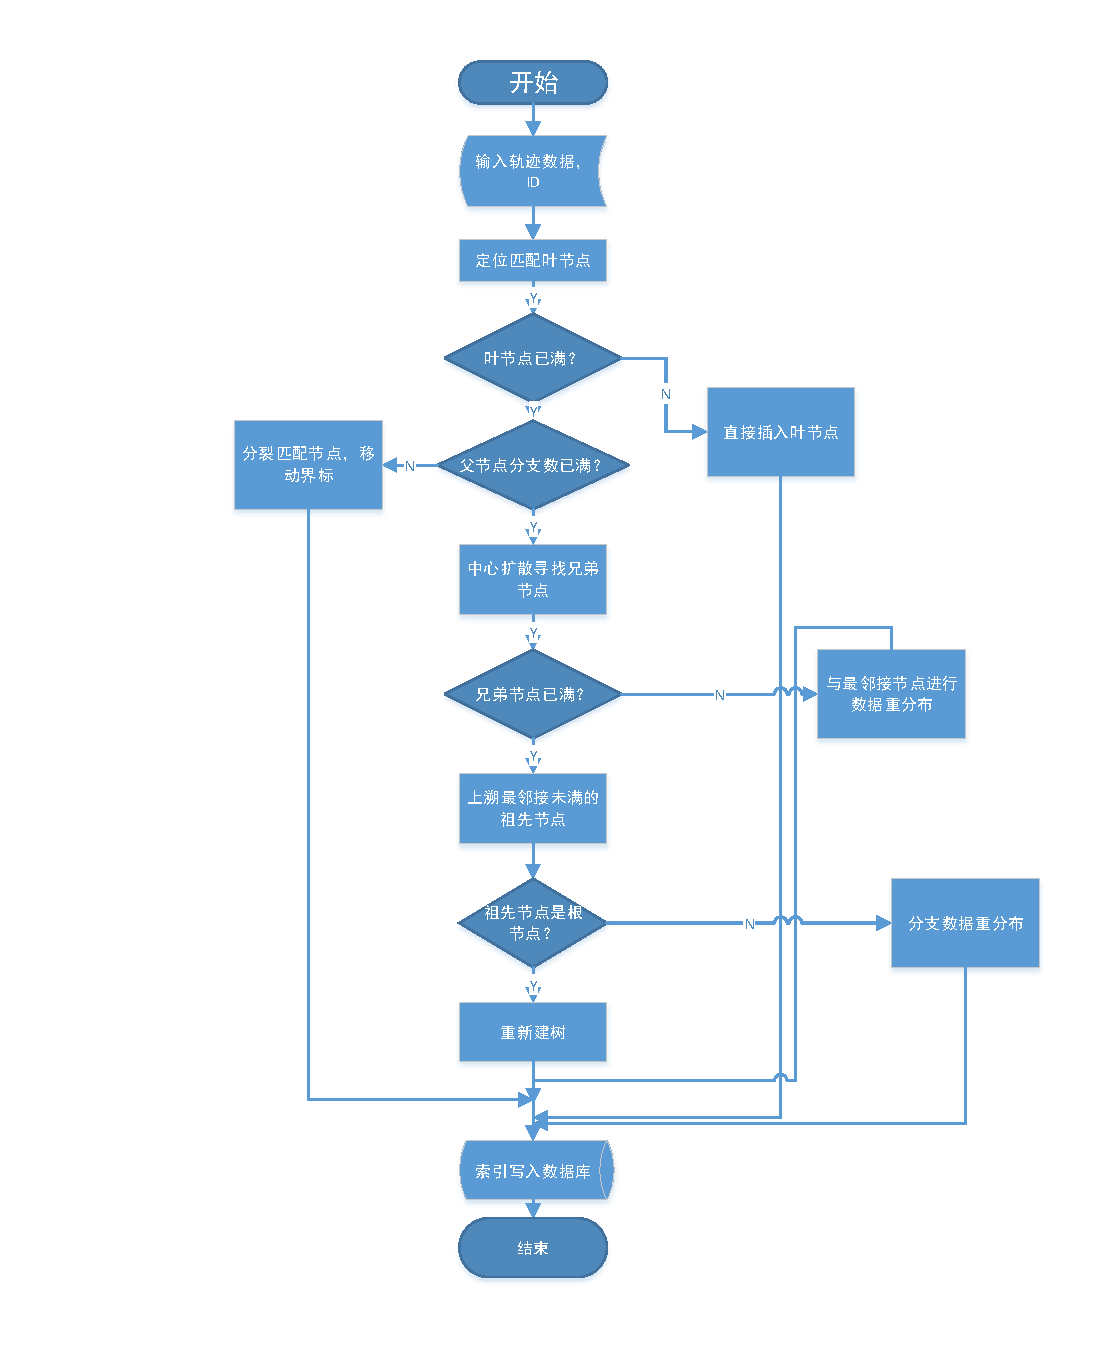
\includegraphics[width=6in,height=6.8in]{new_FIGs/chapter4/vp-tree-insert-flow.pdf}
  \caption{Insert算法流程图}\label{vp-tree-insert-flow}
\end{figure}
\subsection{插入算法实现}
\textbf{已满叶节点的分裂代码实现}
\begin{figure}[H]
  \centering
  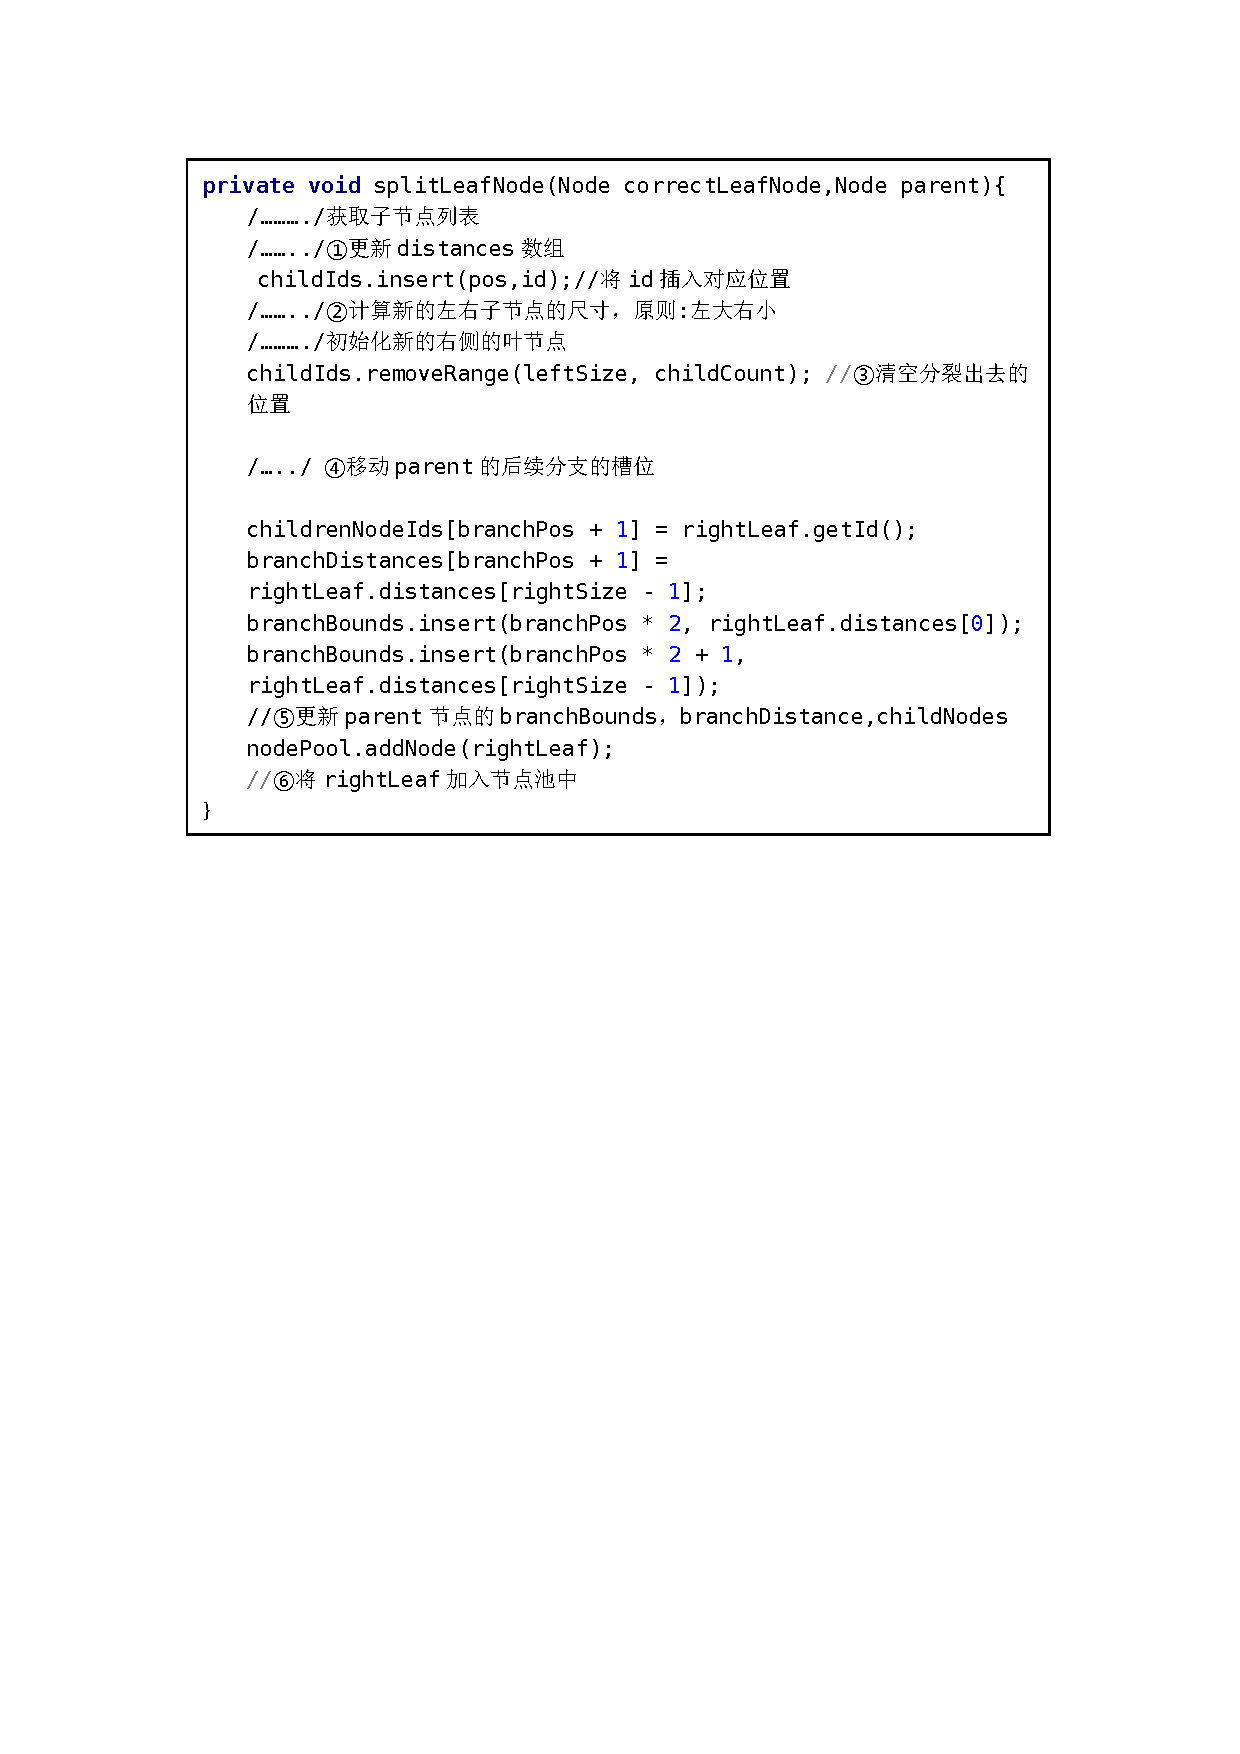
\includegraphics[width=6in,height=7.5in]{new_FIGs/chapter4/insert-code1.pdf}
  \caption{已满叶节点的分裂代码实现}\label{fullleafnode-split}
\end{figure}

\textbf{叶节点数据重分布代码实现}
\begin{figure}[H]
  \centering
  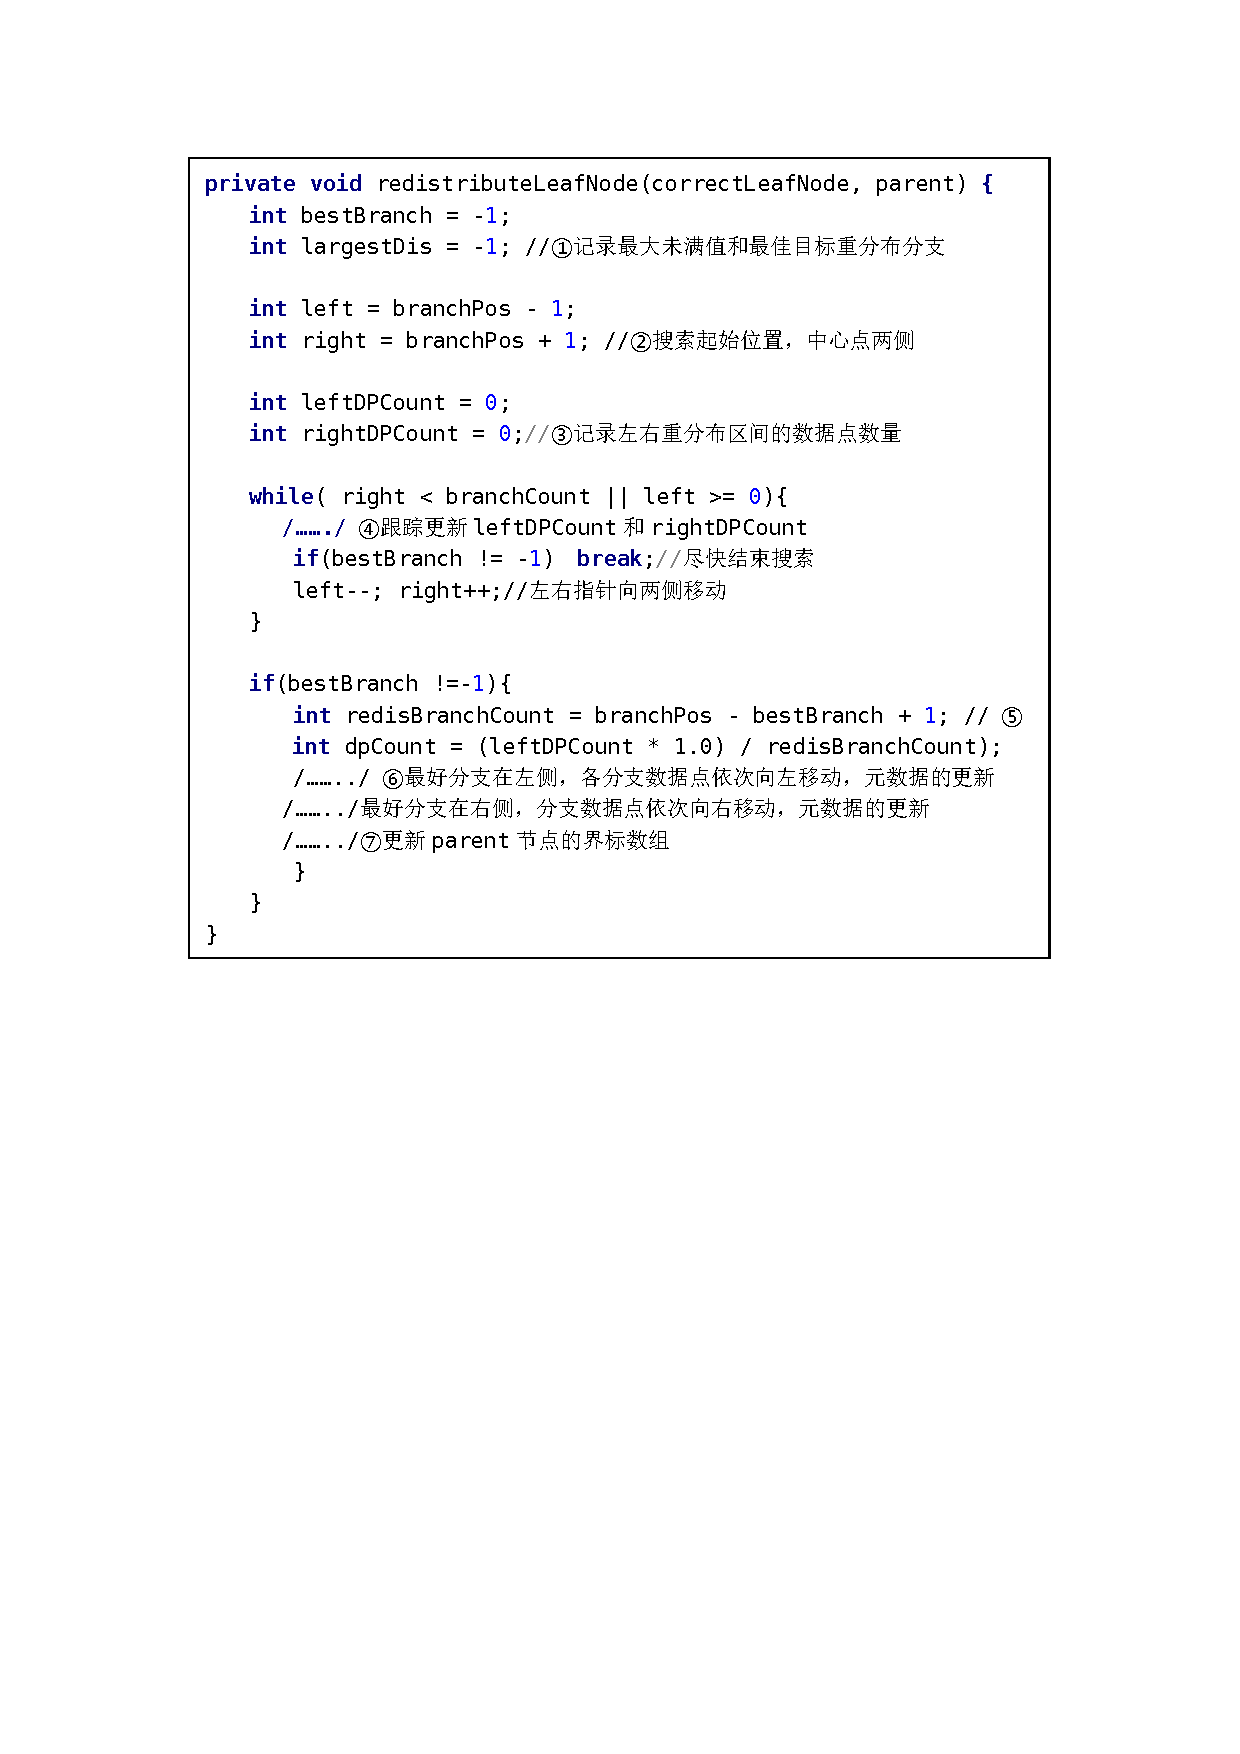
\includegraphics[width=6in,height=7.8in]{new_FIGs/chapter4/insert-code2.pdf}
  \caption{叶节点数据重分布代码实现}\label{leafnode-redistribute}
\end{figure}

\textbf{分支分裂代码实现}
\begin{figure}[H]
  \centering
  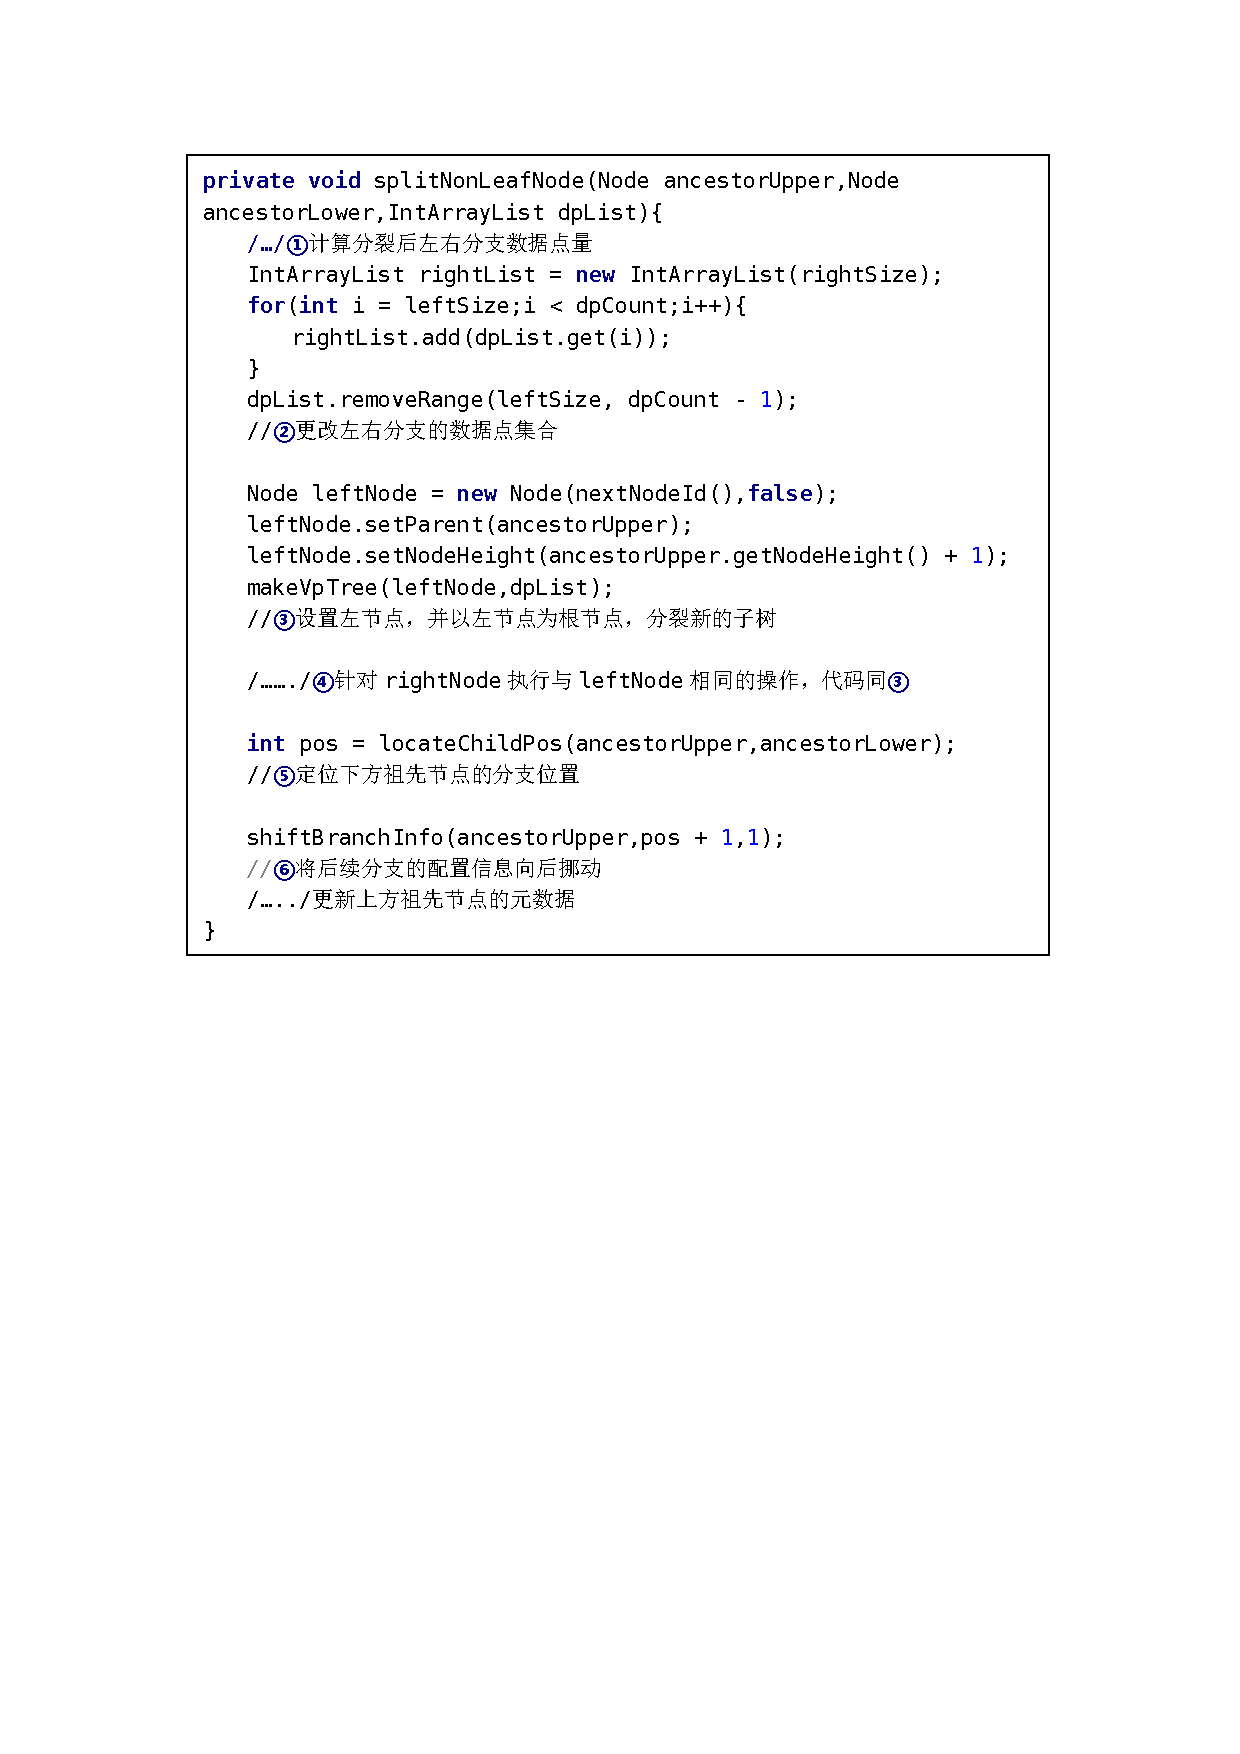
\includegraphics[width=6in,height=6.8in]{new_FIGs/chapter4/insert-code3.pdf}
  \caption{分支分裂代码实现}\label{branch-split}
\end{figure}
分支分裂与叶节点分裂最大的不同,就是必须对分支所拥有的数据点集合进行重新建树。如图\ref{branch-split}所示的,makeVpTree方法其实是createNode方法的封装实现,其目的都是以某一节点为根节点建立子树。而分支配置信息的移动函数shiftBranchInfo的实现与前文所现一致,此处省略,不再展示。
\section{豪斯多夫距离计算设计}
在轨迹数据服务设计的最后,我们介绍豪斯多夫距离计算的设计和实现。这一节相对于本大节的其他内容比较独立,所以用单独的类图予以诠释。
\begin{figure}[H]
  \centering
  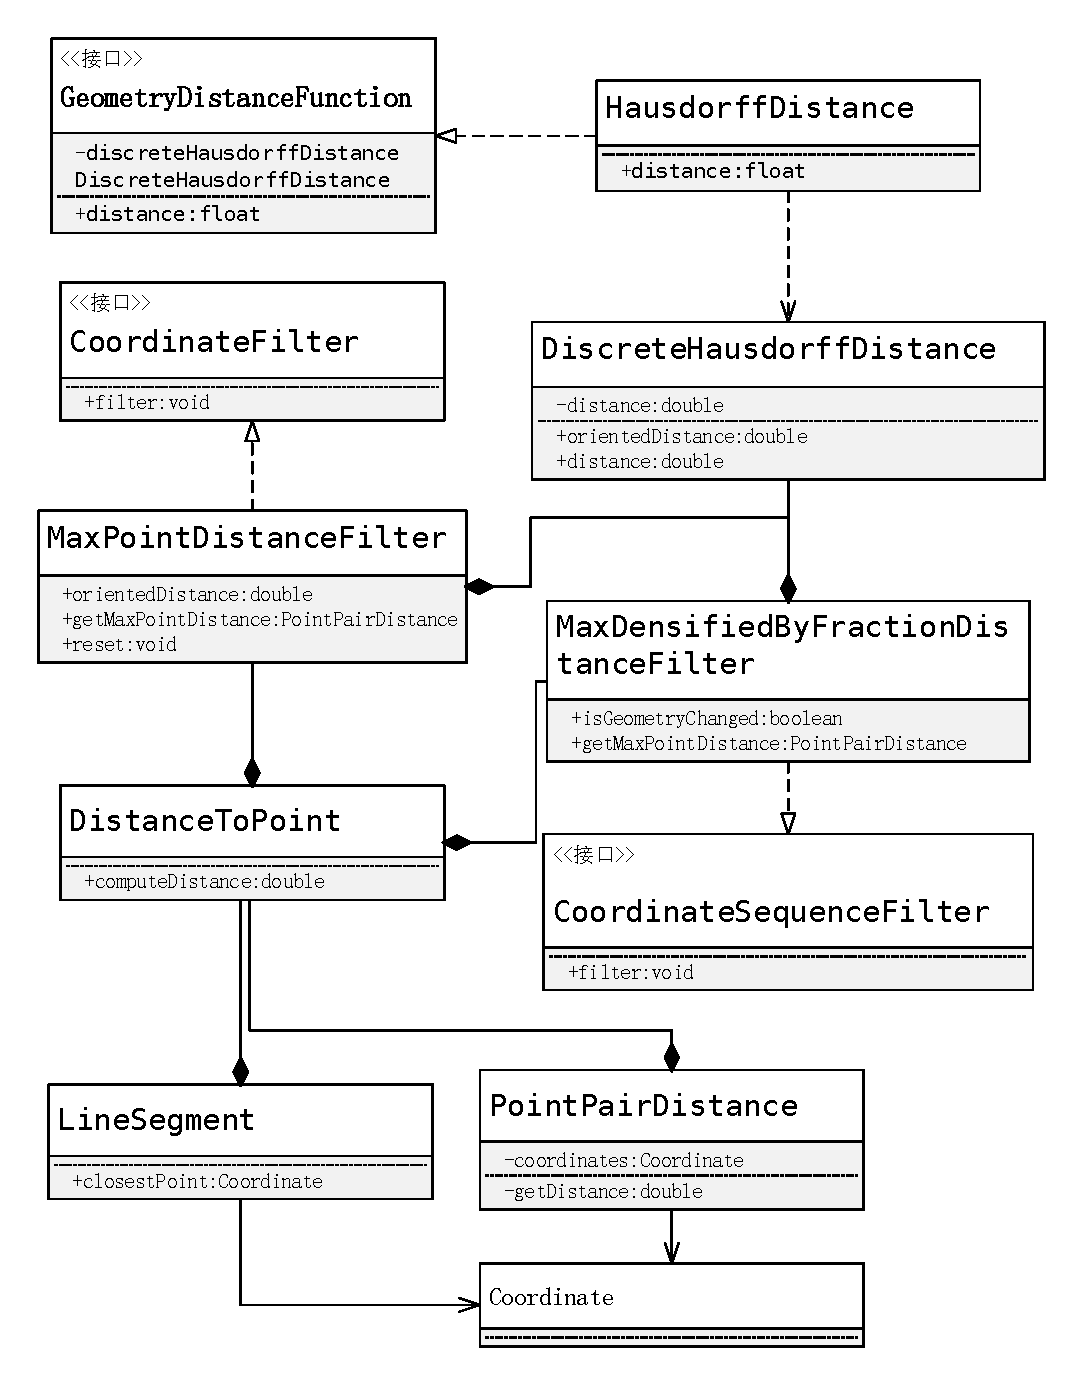
\includegraphics[width=6in,height=6.5in]{new_FIGs/chapter4/hausdoff-dis-class.pdf}
  \caption{轨迹距离计算设计类图}\label{trajectory-distance-compute-class}
\end{figure}
本文主要针对Geometry类中LineString(线条)和Polygon(几何体)两种类型进行设计,因为轨迹数据基本上都属于这两种类型。如图\ref{trajectory-distance-compute-class}所示,HausdoffDistance是对GemotryDistanceFunction接口的实现,它依赖于DiscreteHau \\ sdorffDistance进行离散点豪斯多夫距离的计算。DiscreteHausdorffDistance聚合了两个MaxPointFilter和MaxDensifiedFractionDistanceFilter,这两个是原生JTS.G\\eometry的保留接口,本文对其进行了重写,以实现对最大距离点的过滤作用。DistanceToPoint是数据点距离的计算类,其所依赖的是Coordinate类的坐标距离计算实现。LineSegment是本文对原生JTS.LineSegment的重写,覆盖了closestPoint方法。PointPairDistance是保留两个坐标点之间距离的类。\textbf{在豪斯多夫距离计算的过程中,坐标点之前的距离是二维欧几里得距离。因为本文暂时只考虑平面轨迹。}
\subsection{豪斯多夫距离计算实现}
\begin{figure}[H]
  \centering
  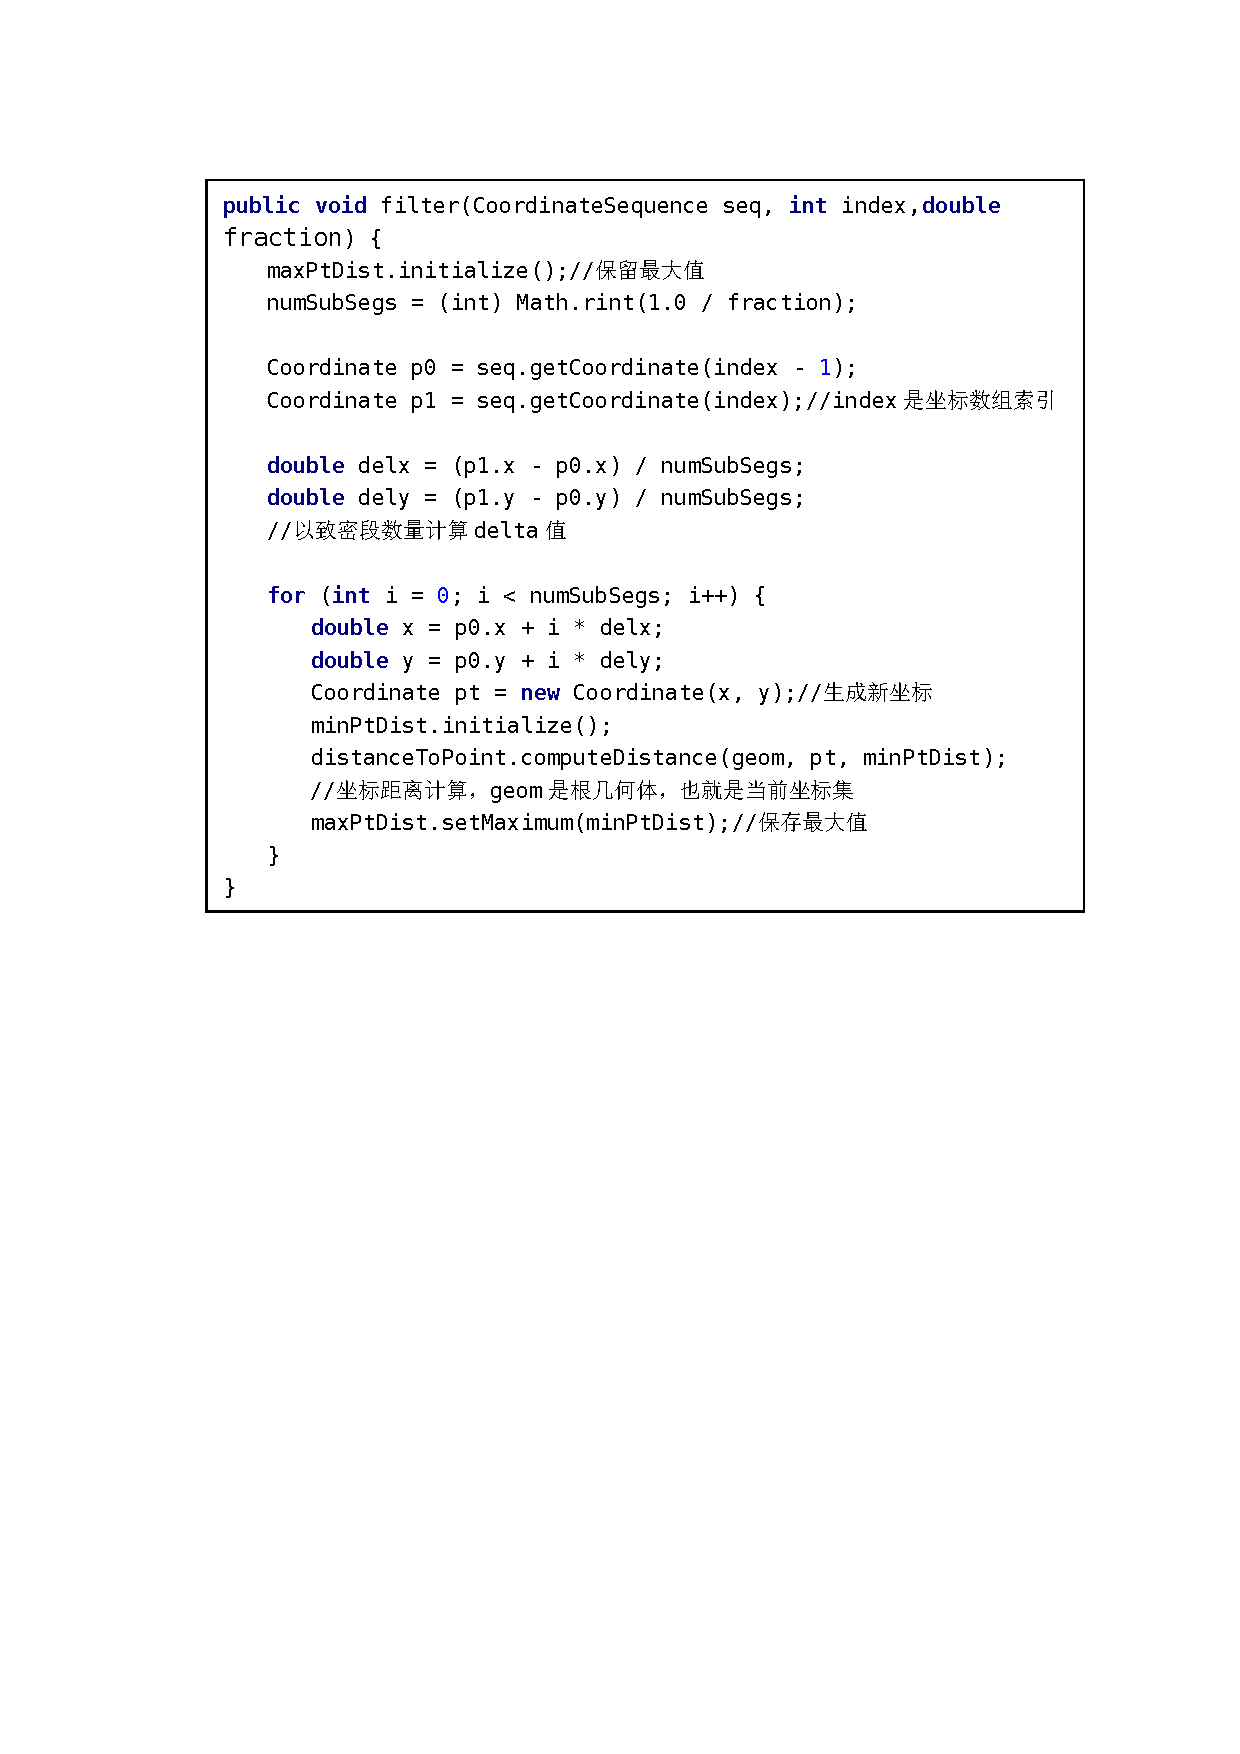
\includegraphics[width=6in,height=4.5in]{new_FIGs/chapter4/hausdoff-code-fraction.pdf}
  \caption{线条分段致密计算代码实现}\label{hausdoff-code-fraction}
\end{figure}
对于前文所提到的点集合全集与目标的距离计算无法实现的问题,本文采用了致密分段这个方式进行这种,代码如图\ref{hausdoff-code-fraction}。原理如图
\ref{hausdoff-fraction-show}所示,致密分段的核心思想是将一根线条按照致密比例切分成数段,将每一段的两端点坐标纳入距离计算,从而尽可能地保留了整根线条的距离属性。很显然的是,致密度越小,致密段数越多,对原线条的距离属性保留越完善,距离也就越精确。但是相应地,运行代价越高,性能越差。
\begin{figure}[H]
  \centering
  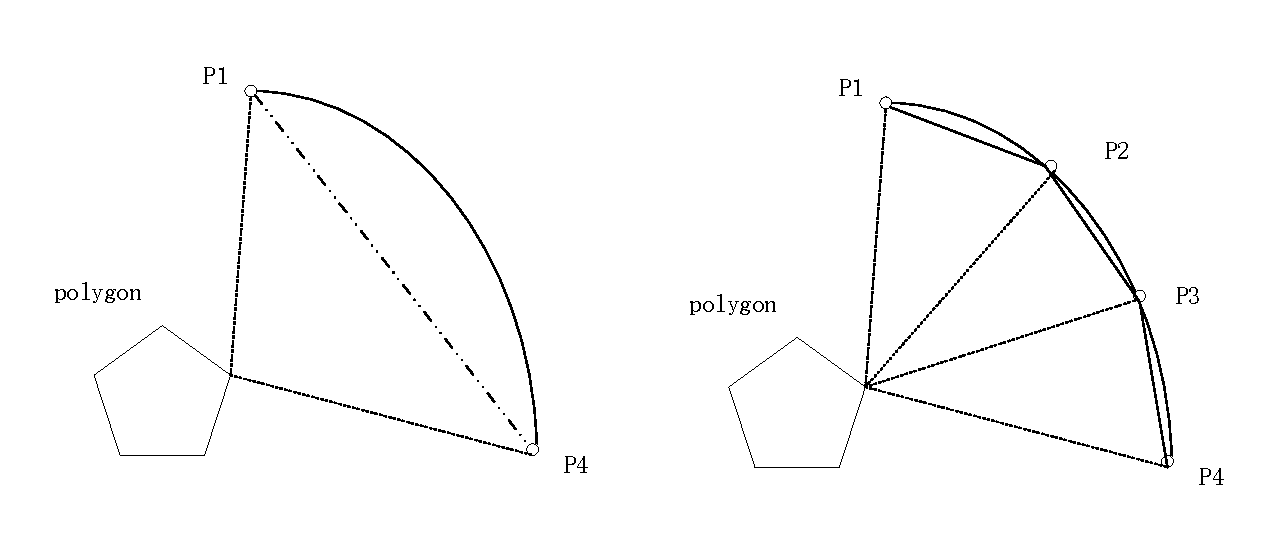
\includegraphics[width=6in]{new_FIGs/chapter4/hausdoff-fraction-show.pdf}
  \caption{线条分段致密原理失意}\label{hausdoff-fraction-show}
\end{figure}
实际上,对于根几何体与目标坐标点的距离计算也采用了类似的分段致密策略进行近似。由于代码类似,本文不再赘述。

\section{本章总结}
本章描述了轨迹数据服务的详细设计和实现,主要介绍了Vptree初始建树,相似轨迹检索以及新轨迹数据插入这三个功能模块的设计要点和原理。通过流程图,类图来说明设计的思路,然后通过具体代码展示关键的实现细节。
